\documentclass[a4paper,oneside,openright,12pt]{report}
\usepackage{graphicx}
\usepackage{xspace}
\usepackage{url}

% font and encoding setup
\usepackage[utf8]{inputenc}
\usepackage[T1]{fontenc}
\usepackage{newcent}

% references
\usepackage{prettyref}
\newrefformat{cha}{Chapter~\ref{#1}}
\newrefformat{sec}{Section~\ref{#1}}
\newrefformat{tab}{Table~\ref{#1}}
\newrefformat{fig}{Figure~\ref{#1}}

% page setup
\usepackage[margin=1.5in]{geometry}
\usepackage{fancyhdr}
\usepackage{setspace}
\raggedbottom
\renewcommand\footnoterule{\vfill\hrule\vspace{6pt}}

% set up floats
\usepackage[font=small,labelfont=bf]{caption}
\renewcommand{\topfraction}{.8}
\renewcommand{\bottomfraction}{.8}
\renewcommand{\textfraction}{.2}
\renewcommand{\floatpagefraction}{.8}

\newcommand{\note}[1]{\marginpar{\begin{tiny}#1\end{tiny}}}
%\suppressnotes

% ignore Overfull \vbox messages
\vfuzz 2pt

\clubpenalty=9999
\widowpenalty=9999
\interfootnotelinepenalty=9999

\newcommand{\vs}{vs.\xspace}
\newcommand{\etc}{etc.\xspace}

\begin{document}

% front matter

\pagenumbering{roman}
%%%%%%%%%%%%%%%%%%%%%%%%%%%%%%%%%%%%%%%%%%%%%%%%%%%%%%%%%%%%%%%%%%%%%%%%%%%%%%%
% Title Page

\pagestyle{empty}
\begin{titlepage}
\begin{center}
\vspace*{\fill}

\huge
Storage for Flexible Commodity Computation
%Serving Files in Service Clusters

\vfill
\vfill

\huge
Russ Ross\\[6mm]
\large
Wolfson College

\vfill

\includegraphics[width=70pt]{eps/camshield}
\vfill

\large
A dissertation submitted to the University of Cambridge\\
for the degree of Doctor of Philosophy

\vfill

October 2006

\vspace*{\fill}
\end{center}
\end{titlepage}
\cleardoublepage

\pagenumbering{roman}

%%%%%%%%%%%%%%%%%%%%%%%%%%%%%%%%%%%%%%%%%%%%%%%%%%%%%%%%%%%%%%%%%%%%%%
% Preface Page

\chapter*{Preface}

\noindent This dissertation is the result of my own work and includes nothing which is the outcome of work done in collaboration except where specifically indicated in the text.

\noindent This dissertation is not substantially the same as any I have submitted for a degree or diploma or any other qualification at any other university. No part of this dissertation has already been, or is currently being submitted for any such degree, diploma or other qualification.

\noindent This dissertation does not exceed sixty thousand words.

\vfill

\noindent This dissertation is copyright \copyright~2006 Russ Ross

\cleardoublepage


%%%%%%%%%%%%%%%%%%%%%%%%%%%%%%%%%%%%%%%%%%%%%%%%%%%%%%%%%%%%%%%%%%%%%%%%%%%%%%
% Abstract Page

\pagestyle{plain}
\enlargethispage*{60cm}        % Make sure this all fits on one page!

{% Required summary page
% Must include name, college, title, date, and the abstract
% approximately 300 words

% for the separate summary:

% \clearpage
% {
% \thispagestyle{empty}
% \begin{center}
% {
%     \Large \thesistitlebig
% 
%     \bigskip
% 
%     \textit{\large Summary}
% }
% \end{center}
% 
% \hfill Russell Glen Ross\\
% November 2006 \hfill Wolfson College\\
% }

% for the dissertation:

\chapter*{Summary}

% the summary

\noindent Standards in the computer industry have made basic components and entire architectures into commodities, and commodity hardware is increasingly being used for the heavy lifting formerly reserved for specialised platforms. Now software and services are following. Modern updates to virtualization technology make it practical to subdivide commodity servers and manage groups of heterogeneous services using commodity operating systems and tools, so services can be packaged and managed independent of the hardware on which they run. Computation as a commodity is soon to follow, moving beyond the specialised applications typical of today's utility computing.

In this dissertation, I argue for the adoption of \emph{service clusters}---clusters of commodity machines under central control, but running services in virtual machines for arbitrary, untrusted clients---as the basic building block for an economy of \emph{flexible commodity computation}. I outline the requirements this platform imposes on its storage system and argue that they are necessary for service clusters to be practical, but are not found in existing systems.

Next I introduce Envoy, a distributed file system for service clusters. In addition to meeting the needs of a new environment, Envoy introduces a novel file distribution scheme that organises metadata and cache management according to runtime demand. In effect, the file system is partitioned and control of each part given to the client that uses it the most; that client in turn acts as a server with caching for other clients that require concurrent access. Scalability is limited only by runtime contention, and clients share a perfectly consistent cache distributed across the cluster. As usage patterns change, the partition boundaries are updated dynamically, with urgent changes made quickly and more minor optimisations made over a longer period of time.

Experiments with the Envoy prototype demonstrate that service clusters can support cheap and rapid deployment of services, from isolated instances to groups of cooperating components with shared storage demands.}
\cleardoublepage

%%%%%%%%%%%%%%%%%%%%%%%%%%%%%%%%%%%%%%%%%%%%%%%%%%%%%%%%%%%%%%%%%%%%%%
%
% Acknowledgements Page

%\enlargethispage*{60cm}        % Make sure this all fits on one page!
% {
%        %Acknowledgements will go here
%        % acknowledgements

\chapter*{Acknowledgements}

My advisor, Ian Pratt, helped in countless ways to set the course of my research and see it through, demanding rigour and offering many helpful suggestions. Major inflection points in my work always seemed to follow meetings with him. Steve Hand also helped me throughout my time at Cambridge, offering sound advice when needed and sharing his mastery of the research game. Jon Crowcroft read drafts of my dissertations, even taking time from his Christmas holiday to send me feedback.

I was fortunate to be in the Systems Research Group during a time when it was full of clever and interesting people doing good research. Andy Warfield, Alex Ho, Eva Kalyvianaki, Christian Kreibich, and Anil Madhavapeddy have been particularly rich sources of conversation and camaraderie.

I might not have survived the whole experience without Nancy, whose love and constant support provided a foundation for everything else.
% }
%
%\cleardoublepage


%%%%%%%%%%%%%%%%%%%%%%%%%%%%%%%%%%%%%%%%%%%%%%%%%%%%%%%%%%%%%%%%%%%%%%
%
% Contents Page

{
  \parskip 0pt plus 1pt
  \tableofcontents
}

\cleardoublepage

%%%%%%%%%%%%%%%%%%%%%%%%%%%%%%%%%%%%%%%%%%%%%%%%%%%%%%%%%%%%%%%%%%%%%%
%
% List of Figures Page

% \addcontentsline{toc}{chapter}{List of Figures}
% {
%   \parskip 0pt plus 1pt
%   \listoffigures
% }
% 
% \cleardoublepage

%%%%%%%%%%%%%%%%%%%%%%%%%%%%%%%%%%%%%%%%%%%%%%%%%%%%%%%%%%%%%%%%%%%%%%
%
% List of Tables Page

% \addcontentsline{toc}{chapter}{List of Tables}
% {
%   \parskip 0pt plus 1pt
%   \listoftables
% }
% 
% \cleardoublepage

%%%%%%%%%%%%%%%%%%%%%%%%%%%%%%%%%%%%%%%%%%%%%%%%%%%%%%%%%%%%%%%%%%%%%%
%
% Glossary

% \addcontentsline{toc}{chapter}{Glossary}
% {
%   \parskip 0pt plus 1pt
%   %\chapter*{Glossary}
% %  \input{glossary.tex}
% }
% 
%\cleardoublepage

%%%%%%%%%%%%%%%%%%%%%%%%%%%%%%%%%%%%%%%%%%%%%%%%%%%%%%%%%%%%%%%%%%%%%%
%
% Terminology

%\addcontentsline{toc}{chapter}{Terminology}
%{
%  \parskip 0pt plus 1pt
%  \chapter*{Terminology}
%  \input{terminology.tex}
%}

%\cleardoublepage


\renewcommand\contentsname{Table of Contents}
\tableofcontents

\addcontentsline{toc}{chapter}{\listfigurename}
{ \parskip 0pt plus 1pt \listoffigures }

\addcontentsline{toc}{chapter}{\listtablename}
{ \parskip 0pt plus 1pt \listoftables }

\cleardoublepage

% page headings for main body

\pagestyle{fancyplain}
\renewcommand{\headrulewidth}{0pt}
\renewcommand{\footrulewidth}{0pt}
\renewcommand{\plainheadrulewidth}{0pt}
\renewcommand{\plainfootrulewidth}{0pt}

\headheight 15pt

\makeatletter
  \if@twoside
    \lhead[\fancyplain{}{\sffamily\small\textsl{\leftmark}}]{\fancyplain{}{}}
    \rhead[\fancyplain{}{}]{\fancyplain{}{\sffamily\small\textsl{\rightmark}}}
  \else
    \lhead[\fancyplain{}{}]{\fancyplain{}{\sffamily\small\textsl{\rightmark}}}
    \rhead[\fancyplain{}{}]{\fancyplain{}{}}
  \fi
\makeatother

\lfoot[\sl\thepage]{}
\cfoot[]{}
\rfoot[]{\sl\thepage}

\renewcommand{\chaptermark}[1]{\markboth{#1}{\thechapter.\ #1}}
\renewcommand{\sectionmark}[1]{\markright{\thesection.\ #1}}

\pagenumbering{arabic}
\onehalfspace
\parskip 10pt

% main text

\chapter{Introduction}\label{cha:introduction}

This dissertation presents the design and implementation of a distributed file system. The design is motivated by the requirements of a new environment that emerges at the intersection of three trends: the renaissance of machine virtualization as a tool for hardware management, the increasing use of commodity hardware and software for server applications, and the emergence of computation as a commodity service.

Providing computing services for hire is nothing new, but previous offerings have always been on a limited scale, restricted to a specific type of application or tied to the tool stack of a single vendor. Web and email hosting services are commonplace, and many applications like tax preparation software and payroll management are available as hosted services. Numerous frameworks for hosted computing have been proposed \cite{amir,vahdat,tullmann} and commercially implemented \cite{amazon,sungrid,kallahalla}, but these require using a specific distributed framework or middleware that introduces a ``semantic bottleneck'' between the application and the hosting environment \cite{roscoe00}. The only way to make hosted computing a commodity is to convince vendors and customers to agree on a common set of interfaces so that applications can be easily moved from one host to the next and an open marketplace can emerge.

Seeking universal agreement on a new application environment is a daunting task, but one that can be circumvented by using an existing platform that already enjoys wide acceptance: the PC. Machine virtualization technology makes it possible to emulate a standard PC with low overhead, while still controlling the resources clients have access to and giving them a secure, reliable environment. Using virtual machines as basic deployment units gives applications access to standard tools and operating systems, and lets them move more easily from a local testing environment to a remote host, or between competing vendors. A combination of flexibility, compatibility, and manageability makes virtual machines stand out as a commodity hosting container.

In this dissertation, I propose that a platform for a commodity computation service be built on clusters of commodity hardware using virtual machines as the management unit. Designing for clusters introduces scale at the implementation level that platform providers can exploit to reduce costs, support a wider range of applications, improve resource utilisation, and foster an ecosystem of intermediate service providers. Instead of managing a complete tool stack demanding a diverse range of expertise, vendors can specialise in hardware provision and management while still achieving the scale to make it worthwhile and leave room for service differentiation. More specialised services and middleware can exist as a value-added service from the same vendor, or third-party providers can layer their services above the virtualized hardware and sell their software and expertise to end users. In this way, vendors of hosted services can focus their efforts on their core expertise without having to build a widely-distributed network or branch out into hardware management as a prerequisite.

Numerous research and engineering challenges are posed by this environment, but this dissertation focuses on providing storage to hosted virtual machines. Unlike other cluster file systems that focus on parallel computation and other scientific workloads, the Envoy file system proposed here is optimised for the requirements of commodity computation. Managers must be able to migrate running services to balance load and make efficient use of hardware resources, so storage cannot be tied to a specific host. Most virtual machines require private boot images, but some also need to coordinate their efforts through shared storage, with flexible control over shared access. The storage system must offer efficient shared access to images with strong consistency guarantees, but it must also accommodate many private images per machine across thousands of machines.

Forcing clients to start from scratch with each deployment and upload an entire operating system image would be costly and slow, and hosting multiple file system images per machine adds a new multiplier to scaling requirements, particularly capacity scaling \cite{warfield}. Expanding the definition of the environment to include a base of commodity software as well as a commodity hardware interface offers a solution to both problems. A few well-known software distributions can be installed by the vendor and offered to clients as templates that they can customise according to their own requirements. By deliberately injecting redundancy into client images, the storage demands can be reduced to a few template images plus the customisations and other data unique to each client. Besides easing storage demands and making inter-client caching more effective, this ties the cost of commodity computation to the degree of customisation required. Clients using standard tools enjoy lower deployment costs than those requiring extensive customisation, encouraging standardisation through economic pressures without imposing artificial restrictions.

Storage systems are normally measured by their performance, but their suitability to the environment they serve is equally important. If clusters of untrusted virtual machines are to succeed as a commodity computation platform, they must be served by a storage system optimised for the expected workload and with adequate features to make management practical.

\section{Contributions}

The thesis of this dissertation is that clusters hosting virtual machines provide a viable platform for commodity computation, and a file system optimised for that environment can support the commodity computation model by providing useful management features and scaling to accommodate arbitrary numbers of file system images under expected workloads.

The first contribution of this work is a definition of the requirements of a flexible commodity computation environment. Commodities are homogeneous enough to make suppliers interchangeable, and have a large enough market for economic forces to ensure that the cost to clients is directly related to the marginal costs of the product or service. I argue specifically for clusters of commodity hardware as the basis of a computation platform, with computation in a virtual machine as the product offered to customers.

The second contribution of this dissertation is the design and prototype implementation of a file system designed for the outlined environment. It builds on previous work on cluster storage systems, but addresses the management needs and scaling characteristics of a platform supporting many independent clients. It also exploits its environment to use the cheap storage available on commodity machines, reduce complexity by integrating with the virtual machine structure, and reduce capacity requirements by explicitly acknowledging the redundancy resulting from a template-based deployment model.

\section{Outline}

The remainder of this dissertation is structured as follows:

\charef{cha:background} discusses the relevant background, including the state of commodity computation and the developments in machine virtualization that underpin this work. Special attention is given to the extensive body of work on storage systems, with a focus on how storage systems are shaped by their intended environments, and how they relate to the new environment proposed here.

In \charef{cha:motivation} I define the problem of flexible commodity computation, and argue for virtual machines hosted by clusters of commodity hardware as the platform for a computation economy. The first part of the argument is that virtual machines decouple hardware management from software management, encouraging transparent competition and specialisation that is not tied to a particular application domain. The second point is that clusters take advantage of economies of scale and allow unrelated clients to share hosting, where careful management can balance the demands of diverse users and make efficient use of resources. The chapter concludes with a discussion of the role of the storage system in this environment.

\charef{cha:design} presents Envoy, a file system for clusters of virtual machines. Like many cluster file systems it builds a distributed file system above a separate object storage layer. Envoy partitions management of the global namespace along hierarchical lines, assigning control of a \emph{territory} to the machine that uses it most, and territory boundaries are dynamically updated in response to runtime conditions. Objects are cached and served directly by the machine that controls the associated territory, eliminating distributed cache coherency protocols while still permitting cache sharing between clients.

The prototype implementation of Envoy is described in \charef{cha:implementation} and evaluated in \charef{cha:evaluation}. The basic functionality of Envoy is fully implemented, with file systems exported to clients using a Linux implementation of the 9p protocol from the Plan~9 operating system. The evaluation tests the performance and scalability of the prototype, validating the overall design and suggesting possible improvements in specific areas.

Finally, \charef{cha:conclusion} concludes and discusses directions for future investigation.

\chapter{Background}\label{cha:background}

This dissertation builds on the rich body of research and systems that have preceded it. In this chapter I present relevant background material to establish the context of the current work. First comes a discussion of commoditisation within the computer industry and how it relates to the proposal in \charef{cha:motivation} for a commodity computation platform. Next, the current state of machine virtualization---an important component of the proposed platform---is presented with an emphasis on recent systems for the x86 architecture. The chapter then turns to influential storage systems and other work that relates to the Envoy file system described in later chapters.

\section{Commodity computing}

Commoditisation relates to computing in two distinct ways, both of which are relevant here. The first is the general consolidation of PC hardware into a series of commodity parts, which are cheap enough and powerful enough to take over many applications that were the domain of specialised ``big-iron'' hardware in the past. The second is the push to offer computation as a service instead of as a product, where billing is based on work done rather than on hardware and software delivered. This dissertation proposes using clusters of commodity hardware as a platform for offering commodity computation services.

\subsection{Commodity big iron}

The scale of the PC market ensures that the best the semiconductor market has to offer is available for PCs. The difference between cheap commodity hardware and expensive mainframes and supercomputers is in scalability, reliability, and manageability. High-end equipment is designed to offer high bandwidth on buses and I/O channels and to scale through highly-parallel configurations. Redundant components mask some classes of faults, and others can be isolated and repaired without interrupting the operation of unaffected components. While these features could be offered in commodity machines, they add too much cost to be worthwhile in environments where service interruption is more annoying than expensive.

\subsubsection{Networks of workstations}

The proposal for Networks of Workstations (NOW) was an early argument for using networks of smaller computers for large problems instead of seeking parallelism through specialised hardware \cite{anderson95a}. While individual components are less performant, the aggregate capacity of a large collection of machines is immense. Commodity disks may be slow, but accessing them in parallel yields high bandwidth as well as high capacity. Reliability and fault tolerance can be designed as a property of the combined system, rather than being engineered into individual hardware components. This has the advantage of transferring the expense from a per-unit manufacturing overhead to a one-time cost in the software design.

PCs have encroached on the workstation market and the two terms are largely synonymous now. The same trends that prevailed in the mid~90s for workstations continue today, however. Switched networks lead to aggregate bandwidth that scales with the number of hosts. Single-threaded performance on cheap PCs is a significant fraction of that on the fastest server hardware. Disks continue to grow in capacity, but their performance improves at a much slower rate. Performance is best scaled through parallelism, and a collection of many machines that all have cheap disks has the potential to outperform even the fastest single controller or collection of high-performance disks attached to a single machine.

\subsubsection{Clusters}

While workstations in an organisation can be profitably pooled for large jobs, clusters are specially built for that purpose and eliminate the workstation role from a node's list of duties. The basic principles behind clusters were laid down in the 1960s \cite{amdahl}, but the power and affordability of recent commodity hardware has brought clusters to renewed prominence. The same hardware used in high-street PCs powers some of the most powerful computing sites in the world \cite{top500}.

Dedicated clusters have a few advantages over more loosely-organised structures. Nodes are typically housed in a controlled environment with redundancy built into power supplies, network links, and cooling equipment. While many clusters grow incrementally, they are still relatively homogeneous, being built from batches of identical hardware. They are also professionally managed and monitored with central control over all resources, unlike looser amalgamations of machines.

As parallel computing vehicles, clusters are mainly used for large ``embarrassingly parallel''\footnote{See \url{http://en.wikipedia.org/wiki/Embarrassingly_parallel}} problems that can be neatly decomposed into discrete tasks. Google has been prominent among commercial users of commodity clusters, and their search engine architecture is an example of a highly-parallel task. The search index can be cloned to serve many concurrent transactions, and partitioned to split processing for a single query over multiple nodes \cite{barroso03}. Scientific workloads, simulations, and graphics rendering farms are all characterised by repetitive computations over huge data sets, and are similarly well-suited to cluster implementation. Beowulf is a popular system specifically designed for addressing these kinds of tasks on clusters of commodity hardware running Linux or other Unix-like operating systems \cite{ridge}.

These problems are generally large enough to warrant custom software solutions as well as dedicated hardware resources. Management software for clusters usually assumes that the application is trusted and cooperative. Systems like TranSend \cite{fox} and CARD \cite{anderson97} require application software to be divided into discrete application units that the monitoring software can direct. Migrating tasks from node to node and compensating for failed nodes requires cooperation from the application, or interaction with a transaction interface that exposes application semantics. Beowulf \cite{ridge} is a lower-level toolkit, providing libraries of useful tools for building a custom cluster application.

For some classes of problems, clusters dominate as the architecture of choice, with clusters of commodity hardware increasingly winning over clusters of specialised hardware. This dissertation does not seek to supplant them for inherently parallel tasks, but rather to extend their advantages into other problem domains. While clusters are a sound choice for problems requiring the dedicated effort of thousands of machines, they can be an equally viable platform for problems too small to require the undivided attention of even a single node. Clusters are normally built and located for a specific user and a specific task, but they can also be built where conditions are best---perhaps near network interconnect points or where cheap resources abound or a favourable regulatory environment exists; strategic choices can give vendors a competitive edge. The advantages of scale can be brought to bear on small and medium-sized problems, not just on the largest of tasks.

\subsection{Computation for hire}

Computer hardware is cheap enough that most organisations can afford to buy systems with sufficient power for their needs. However, because of the complexity of managing computer systems and the ongoing operating and maintenance costs, this is not always the best way to proceed. Numerous avenues exist for clients wanting to hire computation services instead of owning and managing their own hardware and software.

\subsubsection{Replacing the machine room}

The primary motivation for outsourcing computation as considered here is to reduce or eliminate the role of the machine room. Dedicated server hardware comes with expenses that may outweigh the benefits of local ownership and control.

The most obvious costs are direct: physical space required, electricity consumed, and heat produced. Commodity hardware is cheap enough that these runtime costs may exceed the capital cost of the hardware over its service lifetime \cite{barroso05}. Hardware must either be located at a company site, where appropriate facilities must be installed and internet connectivity hired, or at a dedicated hosting facility, where managing it is more complicated and may require sending staff to a remote location.

Maintaining servers also requires qualified staff, another significant expense. The skills required to manage computer systems are unrelated to the core mission of many organisations, forcing them to develop a sizable technical staff to support operations that have little to do with technology. Running a parallel group outside an organisation's core expertise may lead to additional inefficiencies.

These costs are even less palatable when the computation facilities are only needed intermittently. Unpredictable demand may force planning based on peak requirements, but many costs are fixed and do not drop during periods of low demand. When asked about the expenses of their large computing infrastructure, Jeff Bezos of Amazon claimed that cost from lack of utilisation dominated the costs of power, servers, and people \cite{bezos}.

\subsubsection{Hosted services}

Some services are generic enough to be hosted remotely by specialised providers, who make money by offering the same inexpensive service to many clients. Basic applications like email, payroll management, web hosting, and other common services have already attracted commercial interest. Hosting them locally brings all the negative aspects of managing an on-site machine room, while adding little or no value over using a remote provider.

Hosted software eliminates the need for the client to buy or manage dedicated hardware, and the application is managed by specialists who can amortise fixed costs over a large customer base. Upgrades do not require work from the client, making it practical to keep all customers synchronised and further reduce support costs. The unpredictable demand of individual clients can become predictable in the aggregate, allowing more efficient hardware use.

Similar arguments apply to storage outsourcing \cite{ng}, for those wishing to hire managed storage while retaining local control of applications. Multi-site backups, capacity planning, and other domain-specific concerns can be turned over to a specialist, leaving local staff to focus on the problems unique to the organisation.

Hosted services fit well with the present proposal, which takes the concept a step further by splitting management of hardware from management of software. In the service cluster model advocated here, service providers can focus entirely on their applications, leaving hardware management to a dedicated hosting service. Alternatively, clients can hire software management services from one vendor and hardware hosting directly from another, isolating the specific value offered by a software vendor from the basic operating costs that all software applications require.

\subsubsection{Utility computing}

Application hosting is most practical for widely-used services, where few differences exist between clients. The proposal in this dissertation is a form of utility computing, where hardware resources are made available for custom applications at a cost related to resource consumption. \emph{Utility computing} refers to a range of computing models, with the common characteristic of on-demand resource provision. Hosted services as described above, and grid computing as described below, fall under the umbrella of utility computing.

Existing work focuses mainly on large applications where abundant resources are needed, but not necessarily over a long enough period to justify building a suitable hardware solution. An example is rendering feature-length animated films, which requires vast computing power and complex interactions, but only until the project is finished. Vendors with sufficient resources can manage them like batch processors on early mainframes, assigning hardware to a series of applications that have been suitably prepared for the environment \cite{wilkes04}. HP's Utility Data Center (UDC) \cite{kallahalla} uses virtualization to manage services, much like the service clusters described in \charef{cha:motivation}, but focuses on large projects that can be individually adapted to the UDC environment.

The Collective project also uses virtualization to isolate services, and proposes turning the desktop PCs of an organisation into a pool of utility computing hosts to simplify administration \cite{sapuntzakis03}. To end users, interactive applications and services appear as \emph{virtual appliances} that can be instantiated on a local PC. This allows specialised staff to manage desktop software as well as machine-room applications. Desktop PCs act somewhat like terminals for managed software, but terminals that also host computation for their own clients. In some sense, this is the reverse of other utility computing environments; it delivers managed software services to local hardware instead of offering hosted hardware to run client applications.

\subsubsection{Grid computing}

Grid computing \cite{foster,sungrid} seeks to combine resources in the wide area to provide on-demand computation. Utility computing gets its name from basic utilities like power, water, and sewer service, offering a common service to many clients who pay according to what they use. Grid computing styles itself after power grids, which provide a meshed infrastructure to match power producers with consumers across the boundaries of a single utility.

Pooling the resources of many organisations has the potential to put vast resources at the disposal of clients, but it also introduces new problems. Unlike the cluster environments typical of utility computing, grid applications must communicate over the wide area with its low bandwidth and high latency. This makes the grid model most suitable for highly parallel CPU-intensive jobs, which can be parcelled into discrete units and distributed to remote nodes. Moving from a single, trusted management environment makes security considerations more complex as well.

Grid computing requires special middleware, though using virtual machines to support more general-purpose clients has been proposed \cite{figueiredo03,zhao04}. Even then, poor connectivity makes it slow and expensive to transfer large data sets or share data extensively between nodes. The distribution model of grid computing makes it poorly suited to interactive applications or those that require close cooperation between nodes.

Existing utility computing solutions do little to address the needs of an organisation with a relatively small computing infrastructure hoping to stay out of the hardware management business. A few applications can be outsourced to a service provider, and large jobs can be run on hired hardware, but these systems are only applicable to a small subset of the applications running in a typical organisation's machine room. To achieve the scale necessary to make an offering profitable, vendors have focused on hosting widely-used applications and projects that are already large. This differs from the current proposal, which aims to make hosted computation a commodity service practical for a wider range of client applications.

\section{Virtualization}

Resource virtualization makes it possible to put familiar tools and interfaces in new environments without substantial modifications. Virtual machine abstractions allow standard operating systems to share hardware even when they are designed to assume exclusive control. Virtual disk abstractions provide a block interface like that of a standard disk, but without tying it directly to a single piece of hardware. Virtualization is used for a variety of reasons, but the relevant purpose here is for resource management and sharing.

\subsection{Virtual machine monitors}

IBM VM/370 \cite{gum} first virtualized hardware to support legacy code without modification. Modern commercial systems like VMWare \cite{vmware} and Microsoft Virtual Server \cite{microsoftvm} are often used for similar purposes, allowing standard operating systems to run unmodified as guests in new environments. This is useful for testing labs, which can test applications against a range of software configurations on limited hardware, and for end users who need access to applications from multiple software platforms. While this allows access to a wide range of guest software, it comes at a performance cost on some hardware---including the standard x86 platform---which was not designed with virtualization in mind.

Virtual machine monitors (VMM) work by imposing a thin software layer between the operating system and the bare hardware. Unlike emulators or simulators, VMMs allow code to execute directly on the hardware whenever possible. Certain operations break the illusion of isolation, however, particularly those involving I/O, memory protection, and interrupt management. The VMM must intercept these operations and simulate the desired effects on the virtual machine. If the hardware does not allow the VMM to directly intercept such operations, it must do so using software means, such as code rewriting or emulation. The overhead of such virtualization techniques is highest when I/O operations are frequency, as is common in server applications.

The Xen hypervisor uses \emph{paravirtualization}, where the operating system is explicitly ported to the hypervisor environment. By eliminating expensive virtualization techniques for I/O operations, paravirtualization leads to low overhead even for network and database applications with heavy I/O components \cite{barham}. This does not affect userspace applications, whose I/O operations are already virtualized by the operating system, so unmodified binaries can still be used with the modified operating system. The down side is that paravirtualization does not provide support for systems that are not modified to support it, including legacy systems. The combination of high performance and support for modern commodity systems makes it suitable as a host for a managed platform like the one proposed here. Recent updates to the x86 platform support full hardware virtualization \cite{adams}, allowing unported systems to run as well, although explicit support for the paravirtualized environment is still beneficial in reducing overhead.

Virtualization allows a commodity computation platform to isolate hosted services from each other and allow them to be managed without explicit cooperation at the application level. Multiple guest operating systems can run on the same hardware, and virtual machines can be migrated transparently to balance load, collocate related services, or free a machine for servicing \cite{clark}. Virtual machines can even be frozen and migrated to remote sites \cite{sapuntzakis02}, a deployment strategy used by vMatrix \cite{awadallah} to migrate and replicate specialised internet services.

The IBM zSeries \cite{ibmzseries} platform provides a managed hosting environment for paravirtualized Linux, but it does so on specialised mainframe hardware and ties clients to a single vendor solution. The availability of fast, secure virtualization for cheap commodity hardware opens up the possibility of applying these techniques to create an open commodity market for computation.

\subsection{XenoServers}

A public computing platform requires more than just hosting technology. The XenoServers project \cite{reed,kotsovinos04a} explores the infrastructure required to host network services on a public computing platform. The Xen hypervisor started as part of the XenoServers project, which motivated its emphasis on performance over compatibility with legacy code. Application binaries can run without modification in a paravirtualized system, so the modifications Xen requires only affect the operating system.

The XenoServers project also addresses the problem of helping clients find a suitable host \cite{spence}. Network services may have specific connectivity requirements, especially when being deployed for use by a small group or an individual. For example, a game server connecting a group of players requires low latency to a specific set of clients to support real-time interaction. To support a large number of hosting providers, XenoServers also defines the infrastructure for billing through a trusted third party.

This dissertation is not directly linked to the XenoServers project, but it is related. XenoServers provides much of the general framework for public computing, but it does not specify the architecture for hosts beyond the use of the Xen hypervisor. In this work I propose using clusters of commodity hardware as the basis for public computing, and I offer a storage system suitable for that environment. The Envoy file system proposed here also supports a deployment strategy similar to the one we described as part of the XenoServers project \cite{kotsovinos04b}.

\section{Storage systems}

Storage is a fundamental component of all general-purpose computer systems. A combination of high storage density, random access, and low cost has made magnetic storage on rotating platters the dominant medium for durable storage. The time to access a random byte of data from a disk is typically measured in milliseconds, while for DRAM this time drops roughly six orders of magnitude to a nanosecond scale, and that gap is continuing to grow.

Because disks are so slow, storage systems are designed around the goal of accessing the disk as little as possible, and favouring sequential access to avoid costly seek delays. Effective use of cache is vital to this goal, and specialised storage systems tuned to specific system architectures and expected workloads are worthwhile because of the potential speed gains over more general systems.

Storage systems have been studied extensively, and one purpose of this section is to survey related work that has influenced this dissertation. A second purpose relates to the thesis of this work, which argues that an environment can only succeed with an appropriate storage architecture. The works discussed here are presented in the context of the environments they support, in part to establish a pattern of symbiosis between storage architectures and computation environments. Envoy, the file system introduced in this dissertation, is discussed briefly in this section to relate it to prior work, but details of its design are reserved for later chapters.

\subsection{Local file systems}

Disks are mechanical devices and their performance is limited primarily by the need to physically position the disk head over the correct part of the platter to access data. File systems designed for local disks achieve performance by minimising the physical movement required. Disk access can be reduced through caching, and hardware latency can be minimised by arranging data on the disk to minimise movement. Correctness and reliability tend to trump performance as design considerations, however, and the wide variety of possible workloads makes it difficult to pick clear winners from competing designs.

The Berkeley Fast File System (FFS) was the first to optimise data layout for performance by clustering related information. Block metadata is distributed across the disk to be near the file data it describes, file metadata is grouped for files in the same directory, and blocks in the same file are grouped whenever possible \cite{mckusick}. \emph{Clustering}, as this design is called, exploits concepts that extend beyond local file systems: the same expectations of correlated access can be exploited to reduce latency when accessing data across the network \cite{amer}.

File system tracing reveals how files are accessed in real systems \cite{ousterhout}. Most files accessed are small, but size distributions are skewed enough that most data transferred is from large files. Writes are less common than reads, and most files are short-lived. Files access is typically sequential, and most files are read from or written to in their entirety. These trends have proved resilient over time, though the scale has increased and the largest files in typical systems have grown much larger \cite{ruemmler,gibson98b}.

As cache sizes grow, more requests can be satisfied without consulting the disk, and designs can assume that many read requests can be served from memory. All writes whose effects are not quickly undone have to go to disk eventually, so despite being less frequent overall, writes requests can dominate the mix of operations that penetrates the cache and reaches the disk. Furthermore, updates often involve metadata changes as well, potentially requiring multiple costly disk seeks even for small updates.

\emph{Log-structured file systems} (LFS) address this problem by borrowing from database design and making the entire file system an append-only log. Writes are gathered and written as sequential chunks on disk, with relevant metadata rewritten instead of updating existing structures directly \cite{rosenblum}. \emph{Journaling} file systems apply the same idea to other file system types, logging only the intent to update metadata. Once the log is committed, the conventional structures can be updated asynchronously while still guaranteeing durability in the face of a system crash \cite{hagmann,sweeney,tweedie}. Breaking the chain of synchronous metadata commits is also the objective of \emph{soft updates}, a technique that involves careful rearrangement of data in the buffer cache to permit delays and reordered writes \cite{ganger94}.

Studies comparing FFS with LFS \cite{seltzer95} and journaling with soft updates \cite{seltzer00} reveal a complicated picture. Transaction workloads force frequent synchronous writes to support their own semantics, negating the benefits of aggregated writes, and updates to clustered file systems reduce the ordered-write problem enough to keep it competitive with LFS for small file updates. Very different strategies can lead to comparable results, but for all local file systems it is careful attention to the motion of the disk head that leads to good performance.

\subsection{Client-server file systems}

If local file systems can be characterised by how they manage disk head motion, distributed file systems are dominated by concerns of data placement and cache management. For a single host, cache management is easy. The OS has a monopoly on the disk and can reconcile any concurrent requests. Complications are mainly concerned with deciding when to commit writes to disk to ensure durability in the face of a system crash. Distributed systems must also consider consistency between caches on multiple machines. If a cache delivers an out-of-date version of a file, the application may be led to produce incorrect results.

The Sun Network File System (NFS) was the first widely used file system for sharing files across hosts \cite{sandberg}. NFS serves many clients from a single access point (typically a server or a dedicated storage appliance \cite{hitz}), which hosts the persistent and canonical version of a file. Cache policy is unspecified, with no explicit support from the server. Clients generally cache reads and writes in memory and check with the server before relying on old cache entries (typically in the range of 10s of seconds). Thus an update made by one client is only detected by another when the first has sent the update to the server and the second has checked for an update. Clients can send a constant stream of \texttt{stat} requests to check for updates, but they cannot hasten a delayed update from another client, so they can never be assured of having the latest version of a file. An update to the protocol helped reduce traffic somewhat by performing implicit \texttt{stat} requests and including the results with common operations \cite{pawlowski,callaghan}, but the fundamental problem remains as clients still delay writes to the server. The latest update, NFSv4, includes features to improve cache management for uncontended data by \emph{delegating} complete control of individual files to clients and \emph{revoking} the delegation when other clients seek concurrent access, at which point it reverts to the consistency semantics of earlier versions.

Other client-server systems address the problem in different ways. The Andrew File System (AFS) \cite{satyanarayanan85,howard} uses the client's disk as a persistent cache with \emph{close-to-open} semantics. In this scheme, the cache is validated at file open time, and changes forwarded to the server at file close time. To reduce validity checks at file open time, a client can be given a \emph{callback}, meaning that it can assume the file is current unless explicitly notified by the server. These changes improve scalability by enlarging the effective cache size on clients and reducing the load on the server, but they still leave open the possibility of conflicting updates by multiple clients. Coda extends AFS to explore the problem of conflict resolution, opening up access to mobile users and allowing clients to continue operating when disconnected from the network \cite{satyanarayanan90,mummert}. DEcorum goes the other way, extending AFS to strengthen cache consistency using \emph{token passing}---a scheme where each file has a single logical token that a client must obtain before it can write to the file---as well as to interoperate better with existing file systems and reduce recovery time after a crash \cite{kazar}.

The Sprite team observed that---despite the popularity of NFS---few applications explicitly address inconsistencies introduced by the file system, so loosening consistency guarantees in favour of performance gains is a dangerous tradeoff. They sacrificed some performance for full cache consistency by disabling caching for files under contention \cite{baker91,nelson,welch}. Since concurrent access is relatively rare \cite{kistler}, this does not pose a significant problem for overall performance.

In all distributed file systems that permit sharing, there must either be a canonical version of the file (or block \cite{mcgregor}) or some way to reconcile conflicting updates \cite{kistler}. In the former case, some participant is usually nominated as the owner of a particular file through a lease \cite{gray89}, token passing \cite{burrows,mann,kazar}, or some other scheme. Any other host wanting access to the latest version must coordinate through the owner. Ownership may go to the host that provides storage, the one actively using the file, or a management host that connects the two \cite{blaze,keleher}. In Envoy, ownership goes to an active user, which then acts as a synchronous server to other users. Unlike Sprite, the principal user can continue to cache the file locally and share its cache with other concurrent users.

Another possibility is to disallow write sharing. The Cedar file system \cite{schroeder} makes all shared files immutable, and turns the problem into one of versioning \cite{gifford}. Venti takes this a step further by storing all file versions permanently and addressing them by a hash of their contents \cite{quinlan}. Since files are never changed or deleted, the store collects a complete history of all historical states of the file system. In workstation environments, it is possible for storage capacity to grow faster than storage is consumed, making this a feasible system, or past versions can be selectively removed as in the local file system Elephant \cite{santry}.

A less drastic approach is to permit snapshots \cite{hitz}, then mark historical versions as read-only with no requirement for cache coordination \cite{warfield}. Envoy employs this dichotomy between active and read-only file versions, implementing cache management only for mutable objects. It does not coalesce identical read-only objects like Venti or Farsite \cite{douceur02}. It could be extended to do so using a lazy, asynchronous process, but it reduces the need by promoting file system forking with copy-on-write as a management tool to avoid creating many of the duplicates in the first place.

Where snapshot systems typically use copy-on-write to transparently combine old data with new, some systems allow explicit stacking of file systems. Spring \cite{khalidi} allows file systems to be layered with optionally synchronised updates as a mechanism for extending functionality by layering in new features. Plan~9 \cite{pike90} allows any file system mount to be layered over another and their contents combined to give each user a custom view of local and remote file systems \cite{pike92}. The copy-on-write NFS server I developed for the XenoServers project \cite{kotsovinos04b} allows layering instructions to be put in a file in any directory, directing the server to immediately reconfigure the user's view of the file system. These systems can be used as a way to fork a file system, by sharing the common base image and capturing changes in a private layer. Over time this can lead to complex hierarchies of layers, and such systems rely on the semantics of their backing file systems. Envoy can be used in conjunction with a stacking layer, but it already provides explicit support for snapshots and file system forks.

\subsection{Serverless file systems}

While creative caching can alleviate the problem somewhat, all client-server architectures have inherent scaling problems. As a single point of contact for all clients, a server is subject to load that grows in proportion to the number of clients, and it also represents a single point of failure. In addition, the duties of a server tend to make it unsuitable for other uses, so such an architecture calls for a dedicated server. As workstations have grown in power, harnessing their excess capacity to cooperate on large problems has become increasingly attractive \cite{anderson95a}.

In xFS, the traditional roles of a server are split and distributed to the clients to yield a serverless architecture \cite{anderson95b}. Hosts can act as clients, managers that coordinate data placement, and/or storage servers that provide disk space, similar to the file system of the earlier LOCUS distributed operating system \cite{walker}. Cache coherency is achieved through an explicit consistency protocol where conflicting client requests are detected and managed.

In addition, the xFS team observed that modern networks make retrieval from a peer's cache faster than from a disk \cite{dahlin94b}, so sharing and coordinating cache across hosts can yield benefits over independent local caches \cite{dahlin94a}. The resulting protocol was so complex that the team had to employ a formal protocol verifier to get a working implementation \cite{wang98}. While a valid way to manage complexity, reducing complexity through design may be preferable, especially in storage systems where correctness is paramount.

Farsite also targets a workstation environment, but assumes that participating machines are not trusted \cite{adya}. This requires encrypting data and using complex Byzantine agreement protocols instead of trusting hosts that have been assigned management roles. It also calls for a higher replication factor to guard against malicious attacks as well as hardware failures \cite{dahlin94a}, and makes cache sharing between hosts less practical. These restrictions are imposed by the environment, again highlighting the importance of matching storage design to expected conditions.

The downside of having workstations double as servers is that the server function is not completely isolated from the other activities of the workstation. Server load is normally determined by the aggregate activity of many clients instead of that of a single unpredictable user, and a user may also switch a workstation off without notice. While a server can also fail unexpectedly, careful administration generally makes this an infrequent event. Extra redundancy is necessary to make files \emph{available}, even when they are still reliably stored on a workstation that has been powered down.

The same trends that lead to excess capacity in workstations make dedicated servers cheap and powerful, without the additional complexity of a heterogeneous management environment. Despite numerous studies showing feasibility \cite{bolosky,douceur99,douceur01} and systems developed and tested \cite{adya,walker}, no serverless file system has seen widespread use for general-purpose computing.

While Envoy has similar goals for serving a location-independent file hierarchy to many untrusted clients, putting it in a trusted cluster environment changes the assumptions significantly. Hardware virtualization allows malicious clients to coexist on hardware with trusted server processes, and the complexity of Byzantine failure models can be avoided. Managed hardware also means that replication factors can be planned around hardware failure rates and load balancing without worrying about hosts being switched off by desktop users.

\subsection{Wide-area file systems}

Carrying the idea of distributed file systems to the logical extreme leads to global file systems, running on hosts throughout the world and serving millions of clients located anywhere. Latency and available bandwidth become major concerns in this environment, and the inability to trust hosts forces widely-distributed file systems---as was true with Farsite in a smaller setting---to focus mainly on managing replicas for availability and reliability.

\subsubsection{Systems with servers}

Ficus \cite{guy} and Echo \cite{birrell93} link servers together to form a single, global file hierarchy, with transparent navigation between the discrete volumes that make up the system. In Echo, entire volumes are replicated in tightly-synchronised groups with one \emph{primary} server and one or more \emph{standby} servers. A token-passing scheme allows clients to cache files locally but still maintain global consistency \cite{mann}. Ficus relaxes the synchronisation requirements in favour of optimistic concurrency, where conflicts must be resolved after being detected. Volume replicas are loosely synchronised, and each may hold copies of only a subset of the files logically contained in the volume. Updates can be made to any file that has at least one replica available \cite{popek}, permitting continued operation in the face of network partitions or other failures, similar to Coda \cite{kistler}.

An early version of xFS \cite{wang93} also follows a two-tier model, where loose clusters of nearby hosts work together and share a single \emph{consistency server}. The consistency server acts as a proxy for the group when communicating in the wide area, and as a coordinator for operations within the cluster. Requests are served from the cache of a local host when possible, and forwarded to a remote cluster when necessary. Consistency is maintained through tokens that permit local caching for multiple readers or a single writer. To reduce the state that must be tracked, tokens cover entire groups of files.

JetFile \cite{gronvall} and Pangaea \cite{saito02a} rely on pervasive replication with little overall structure. JetFile  uses specialised servers for a few metadata functions, but most operations happen directly between clients. In both systems clients maintain replicas of all files they are interested in, and optimistic concurrency control permits disconnected operation. They differ in how updates are propagated. Pangaea maintains a replica graph for each file and pushes updates to other clients \cite{saito02b}, while JetFile makes extensive use of IP multicast to locate replicas and announce changes, and clients pull updates when required. When conflicting updates are detected in either system, the versions must be reconciled explicitly, generally using a last-writer-wins policy.

\subsubsection{Peer-to-peer systems}

Relying on trusted servers restricts the audience for a wide-area file system to large organisations and service providers who can maintain widely-dispersed networks. Peer-to-peer systems use resources volunteered by participants on large numbers of machines.

The simplest systems are read-only file distribution schemes. Bittorrent tracks all clients with a central manager, but data blocks are transferred mainly between clients \cite{cohen,pouwelse}, which request blocks they have not yet received from peers that have already downloaded them. Avalanche \cite{gkantsidis} uses network coding to decrease the incidence of ``rare'' blocks that make it difficult for clients to complete the last steps of a file download. Both systems feature capacity that grows with the number of users, without consuming excessive bandwidth at the server. Such systems are mainly useful for sharing the cost of distributing static content with those who benefit from it, and not for general-purpose storage needs.

\emph{Distributed hash tables} (DHT) such as CAN \cite{ratnasamy}, Pastry \cite{rowstron01b}, Chord \cite{stoica}, and Tapestry \cite{zhao01} provide distributed lookup services on peer-to-peer networks, and have been used as the basis for wide-area file systems. CFS \cite{dabek} and PAST \cite{rowstron01a} implement read-only systems using content-based addressing, similar to Venti \cite{quinlan}, but using an underlying DHT to locate object replicas. Other systems implement mutable file systems over similar substrates, storing data blocks, files, or content-based fragments \cite{rabin81} as immutable objects distributed across the network. Pasta \cite{moreton} stores metadata in special index blocks, each of which is associated with an asymmetric cryptographic key. The key is used to locate the index block (instead of using a hash of the contents as for normal data blocks) and to protect changes to it, allowing the index to change while retaining a unique static ID. Eliot \cite{stein02} stores metadata outside the immutable substrate, creating a separate, writable system that references the read-only data indexed by the DHT. Ivy \cite{muthitacharoen02} stores all user changes to the user's log, which is then made available to others through the DHT, and each user consults as many logs as necessary to construct a coherent view of the file system.

Peer-to-peer file systems all suffer from the transience of users. Volunteered resources can be withdrawn without notice, so high levels of replication are required to ensure accessibility and availability \cite{blake,rabin89}. Latency is also high in the wide area, so further replication and caching is necessary to make performance acceptable. OceanStore \cite{kubiatowicz} was designed as a global network of highly-connected clusters that cooperate closely, with additional clustering at the file level for groups of files that are regularly accessed together. The prototype, called Pond \cite{rhea}, uses Tapestry to organise virtual resources (data blocks and manager nodes), but it also forms localised clusters of participants to implement Byzantine agreement protocols without the high latency typical of DHTs. These systems are tiered to reclaim some of the benefits of locality while still providing a global service.

Envoy has some structural parallels with these systems. While latency between machines in a cluster is much lower, Envoy still caches data on disk and in memory near the client. Locality is pursued at the machine level to aggregate the storage requirements of a set of virtual machines, with data ultimately replicated and spread throughout the cluster as storage objects.

The relationship of the present work to global storage systems is more than just a passing architectural resemblance, however. Envoy and the service clusters that host it are designed for commercial providers that locate computational resources near storage and fast network access. Instead of trying to hide the distance between users and data, service clusters share the goal of XenoServers \cite{reed} to move computation to a resource-rich environment. As a basic platform, service clusters backed by Envoy storage can form the building blocks of global service networks, including storage services.

\subsection{Cluster storage systems}

The path from local file systems to wide-area file systems is generally progressive, with concerns about cache management, trust, latency, replica placement, and reliability growing at each step. Clusters have networks with low latency and high bandwidth, and large numbers of trusted, centrally-managed hosts. Their mixture of characteristics from the largest and smallest of systems partially explains their popularity as replacements for traditional, monolithic supercomputer architectures.

With a large number of redundant components, clusters have the potential to be highly reliable (in the aggregate) with abundant bandwidth. One of the principal drivers of cluster storage systems is avoiding bottlenecks. While this is important in all systems, the vast aggregate disk and network bandwidth available to a large cluster makes it easy to overwhelm any single component \cite{hospodor}. In addition, the opportunity cost of wasted resources is potentially very high, so cluster systems must make good use of the combined storage capacity and I/O bandwidth available from the array of component machines.

\subsubsection{Storage layers}\label{sec:storage-layer-systems}

A common approach for cluster storage systems is to divide the problem into two distinct layers: one that manages the physical disks, balancing load and capacity and handling the addition and loss of disks, and a second layer that builds a file system above an abstract block- or object-level interface provided by the first.

Zebra \cite{hartman93} stripes data across multiple storage servers in a network version of RAID \cite{patterson}, but uses a single file manager to coordinate metadata. Zebra is based on the Sprite LFS implementation, and clients cache data and metadata the same as they would in Sprite. The file manager assumes the role of a standard file server, but all log operations are striped and clients direct data requests directly to the storage servers. Swarm \cite{hartman99} removes the file manager to present a stand-alone layer that exports striped logs to clients, which can be used to implement local file systems or other high-level services.

Petal \cite{lee95,lee96} pools storage devices to export sparse virtual block devices to clients. Persistent state is distributed across the servers, and global state is updated using a distributed agreement protocol that tolerates node failures. By caching a small amount of metadata, clients can direct most requests directly to the correct storage server, updating metadata lazily when it proves to be out-of-date. Petal maintains a global map of servers for each virtual device, optionally using \emph{chained declustering} for redundancy. Chained declustering \cite{hsiao} allows simple load redistribution when nodes fail and makes catastrophic failures more likely to damage a few virtual disks extensively than cripple many virtual disks with small corruptions.

Frangipani \cite{thekkath} builds a file system over a Petal virtual disk. It takes advantage of the large, sparse address space to simplify data structures, with large regions reserved for inodes, allocation bitmaps, logs, small blocks, and large blocks. As with most layered systems, the physical layout is not determined by the virtual layout, so many of the layout strategies of local file systems are inapplicable \cite{stein05}. Instead, the layout of files is simple, with a map tracking up to sixteen 4~KB blocks for small files, spilling into one of $2^{24}$ large blocks that can store files up to 1~TB. File systems can be shared by multiple clients; a distributed lock manager coordinates caching and prevents corruption from concurrent access.

Object-based storage systems \cite{factor,mesnier} provide an object-level interface to disk space. Instead of exporting virtual disks to clients, they manage storage as collections of objects with attributes, which generally correspond directly to files and directories in complete file systems. Network-attached secure disks (NASD) drop storage servers and embed management functions directly in the storage device to save costs \cite{gibson97,gibson98a}, while metadata is controlled by a separate server. They require a separate metadata server to manage security and coordination for shared storage, but cryptographic techniques make these metadata operations largely asynchronous. Synchronous communications are mainly confined to direct requests from clients to the storage devices. 

FAB \cite{frolund,saito04} refines the ideas found in Petal and introduces the idea of \emph{storage bricks}---dedicated storage modules made from commodity components that can be combined to form a storage pool. FAB randomly assigns each data segment to a set of storage bricks and uses majority voting to manage replicas. This allows it to tolerate failures and add new bricks without pausing and temporarily ignore overloaded servers. It also supports fast snapshot operations without a centralised coordinator \cite{ji}.

The Self-* Storage project aims to extend brick-based storage to automate many aspects of configuration and management of storage in order to reduce administrative hassle and costs \cite{ganger03}. Like the AutoRAID storage device \cite{wilkes95}, the Ursa Minor prototype \cite{abd-el-malek} focuses on optimising data layout and failure tolerance for different workloads and requirements. Using a unified infrastructure it supports multiple storage policies and can convert existing data while still operating normally.

Storage layers are complementary to the goals of Envoy. Indeed, the Envoy prototype's primitive storage layer is a stub intended to be replaced by a system much like those described here. Envoy assumes a reliable and performant storage layer, and builds a complete distributed file system optimised for large numbers of untrusted virtual machines above it.

\subsubsection{File systems}

Built on storage layers that can deliver parallel access to many disks, cluster file systems are left mainly with problem of managing metadata and maintaining cache consistency. Lustre \cite{lustre} follows the model proposed by the NASD group \cite{gibson98a}, with clients contacting storage devices directly for object-level data access. Metadata is controlled by a centralised server with a failover replica.

The Google File System \cite{ghemawat} focuses on a specific workload and drops the POSIX file system interface. It, too, splits metadata management from data storage, but is further optimised for large files with sequential reads and append-only writes. Random reads and writes are supported, but the overall emphasis is on high throughput rather than low latency. In this environment, data caching has little value and metadata is minimised by managing files as sequences of large, 64~MB chunks. Chunks are stored as normal files using a Linux file system on commodity hardware.

Clusters are widely used as replacements for supercomputers, and many cluster file systems are tuned to scientific-computing workloads. Like the Google environment, they often require high sustained throughput from large files. Unlike workstation environments where read-write sharing is rare, scientific computing makes frequent use of parallel processes writing to different parts of the same large file \cite{wang04}. GPFS \cite{schmuck} is optimised for large deployments where any centralised coordination point is unacceptable. Based on a block-level storage system, it supports a high degree of concurrency by replacing the centralised metadata manager with a distributed lock manager with byte-range locking, and using extensible hashing to support large directories that can be queried and updated concurrently. In addition, it allows write sharing for non-conflicting metadata updates and pushes most of the communication burden for token revocation to the client triggering it, further reducing synchronous metadata operations in the lock manager.

Many commercial solutions use dedicated storage area networks (SAN) to connect hosts with storage devices over a high-speed switching fabric. As with most of the systems described here, SANs let clients connect directly to storage devices and rely on a separate layer to mediate sharing and form a file system. Storage Tank \cite{menon} uses manually-configured partitions of the namespace to distribute control between metadata servers and relies on the block-based interface provided by SANs, but the overall structure is similar to systems like GPFS.

Ceph \cite{weil06} is also tuned to scientific cluster workloads, but is based on object storage. It, too, distributes metadata management to avoid bottlenecks, but instead of using distributed locks and having clients directly modify metadata structures, it builds a distributed version of the metadata manager common in other object-based systems. Object replicas are placed according to a special hash function, allowing clients to compute the location of an object instead of having to consult the metadata manager. Ceph handles the problem of heavy write sharing in scientific workloads by augmenting the POSIX interface to allow weakened consistency semantics. This works for scientific computing, where applications are generally custom-written anyway, but is less helpful when clients use commodity tools. Like Envoy, Ceph divides management of the hierarchical namespace according to runtime activity, but it does so purely for load balancing within the distributed metadata service \cite{weil04}; no server benefits more than another from controlling a particular region of the namespace. Envoy, in contrast, delegates metadata management to the client dominating access to that part of the file system, making the placement of metadata management a matter of absolute performance as well as load distribution. It also differs from Ceph's distributed scheme by using a time-based protocol to prioritise changes and promote stability (see \secref{sec:territory-management}).

While Envoy is also built for clusters, it is designed for many independent clients with more traditional workloads, rather than large, scientific systems bringing the power of thousands of machines to bear on a single data set. Envoy creates a single hierarchical namespace, but it is arranged as an administrative tree with discrete, client-level file systems as leaves. Envoy is optimised to manage large numbers of these images, with full administration of a private image being managed by the machine using it, and control of shared images being distributed among the participating clients according to runtime demand. In this way, Envoy---with its model of a cluster being host to more clients than machines---is largely complementary to the systems described here, which attempt to make the cluster act like a single, large machine. Instead of centralising metadata management and then introducing distribution schemes to overcome the limitations of centralisation, Envoy partitions the namespace according to runtime demand and distributes metadata control to the clients, or more precisely to a secure virtual machine hosted on the same node as the client.

\subsection{Virtual machines}

A few storage systems have been designed specifically for virtual machine environments. Operating systems hosted on virtual machines can use conventional file systems implemented on private block devices. These can be physical partitions assigned to individual virtual machines, or virtual block devices accessed through a virtualized driver. In addition, network-facing client protocols such as NFS operate the same on virtual machines as on real machines.

My experience with two systems influenced the design of Envoy. The first was CoWNFS, a stacking file system that uses copy-on-write techniques and user-controlled layers to emulate snapshots and file system forks \cite{kotsovinos04b}. CoWNFS operates as a userspace NFS server running in an administrative virtual machine and exporting customised storage views to clients. A private, writable layer can be stacked over a read-only template to capture changes and isolate them from other users. Sharing is possible between clients through the NFS protocol, but access is limited to files already available in the namespace of the administrative VM.

The second system, Parallax \cite{warfield}, exports private virtual block devices to clients. Like CoWNFS and Envoy, Parallax operates through a server in the administrative VM on each host. Template images with fork and snapshot support assist rapid deployment of clients, using a copy-on-write mechanism as clients diverge from their starting templates. Parallax operates at the block level with no support for sharing between clients, except when clients inherit read-only blocks from the same template. A distributed block-storage layer makes use of cheap commodity disks in the host machines for persistence and location-transparent access.

Ventana \cite{pfaff} is a file system for virtual machine environments with similar goals to Envoy. Like Parallax and CoWNFS, both systems provide a single server for each machine, which clients access through a virtual network or block device. Ventana also supports snapshots and forks of file system images, and tracks versioning at the per-file level. Like Envoy, it uses an object-based storage layer, but objects are immutable and changes are tracked through successive file versions, similar to JetFile \cite{gronvall}. Ventana uses a centralised metadata server to track file versions (unlike JetFile, which announces new versions through IP multicast) and to manage image branches. It offers loose consistency, communicating with clients over the NFSv3 protocol and requiring nodes to check with the metadata server on each access to bound cache divergence. Persistent caching at each node permits disconnected operation for clients, and any resulting conflicts are managed by applying all client changes to the repository after making a snapshot. To lessen the bottleneck of a centralised metadata server, Ventana allows file system images to be marked as private and all metadata to be cached at the node. Envoy targets clusters of virtual machines where centralised servers are impractical. Metadata control is distributed, and manual configuration of private and shared images is rejected in favour of dynamic algorithms that adapt to runtime behaviour.

Virtual machines have also been used to support grid computing \cite{figueiredo03}. GVFS \cite{zhao04} extends NFS with userspace proxies that implement persistent caching, file prefetching, and per-file metadata hints, allowing compressed transfers and other deviations from standard NFS semantics to better support the wide-area grid architecture. Like other virtual machine storage systems, GVFS exploits the redundancy in file system images cloned from a template, using symbolic links to introduce some transparency in the cloning process and facilitate shared caching.

\section{Summary}

Amazon EC2 \cite{amazon}

Palimpsest \cite{roscoe03}

Multi-Service Storage Architecture \cite{bacon}
\chapter{Service Clusters}\label{cha:motivation}

The standardization of the shipping container revolutionized the logistics industry, which in turn has had a significant impact on global commerce over the past 50 years. Building a box hardly seems like the stuff of revolutions, but the cheap availability of foreign goods and easy access to global markets that characterizes modern economies owns much to exactly that. The significance of the container is illustrated partly by what it offers, namely, flexibility and efficiency, but equally significant is what it does not offer. It is not an engine, a vehicle, a route, a company, a service, or any of the things necessary to transport goods from one place to another. Instead, it is a neutral, common ground. Those wishing to ship something can pack according to well-known dimensions using widely-available tools, and those offering transport services can use trains, ships, trucks, or whatever method of transport and whatever routing system allows them to offer competitive service while making a profit.

The computer industry is in need of a shipping container. While the computer hardware industry is increasingly viewed as a commodity business, computation as a commodity service is still in its infancy. The components are all there: PCs are powerful, networks are fast, disks are big, operating systems are flexible and efficient, and everything is cheap. The Top~500 supercomputer list is dominated by clusters make from commodity hardware \cite{top500}, and companies such as Google have used commodity hardware to solve large commercial problems instead of relying on powerful, special-purpose hardware that is more powerful and more reliable, but also much more expensive. These efforts have been highly successful, but they still revolve around using commodity hardware to build platforms that are customized for a particular task or class of tasks. Like oil tankers or passenger trains, they are efficient and well-suited to their intended markets, but not easily adapted to other kinds of clients.

Containers have succeeded for several reasons. They are generic enough to support an enormous range of cargo, but rigid enough to pack tightly together and stack neatly. They can be pulled individually behind trucks, strung together on trains, or packed onto huge cargo ships for ocean transport. They can be moved and loaded easily and quickly using cranes, and they can move from one ship to the next without any changes. Clients can fill as many containers as they need and only pay according to what they use.

Many of these same characteristics would help to make commodity computation a reality. Clients should be able to deploy a wide range of computation and communication services, but vendors should also be able to manage them in a generic way. Clients should be able to use their own commodity machines and software to implement services, but have them run equally well in a large, commercial setting. Likewise, deployment costs should be low and procedures simple, and redeployment costs should not create onerous barriers to changing vendors. Finally, small services using very few resources and those spanning many dedicated machines should be able to coexist without interfering with each other and with clients paying according to what they use.

In this chapter I argue that a platform of \emph{service clusters} approximates this ideal, using commodity hardware and commodity operating systems and tools, isolated and managed using virtual machine monitors. The \emph{service} is the unit of management, allowing arbitrary tasks to run, each isolated in a virtual machine. While I do not prescribe a particular operating system or set of tools, I do suggest that a small set of common, commodity platforms can be agreed on, and that clients and vendors can both benefit from adhering to them. Clients can then package their custom services as everything that differs from a standard platform and send it to the vendor that can host it according to their needs.

Not every task is best served by a common platform---oil tankers will continue to excel at transporting oil---but many jobs that today run on custom installations could be better implemented as commodity computation tasks that are cheaper for clients to run and profitable for vendors to host. I discuss other efforts toward commodity computation and how my proposal overlaps or relates to them.

Finally, I do not propose a complete solution. Instead, I argue for the essential characteristics that distinguish service clusters from other large-scale uses of commodity computers, while leaving much of the general infrastructure to others. I focus on the storage needs of the platform and identify how a suitably designed file system can use the commodity hardware in a cluster to cheaply and easily support deployment and management of services built on commodity tools.

\section{Commodity computation}

Services are harder to package as commodities than goods. The quality of oil, the purity of precious metals, the strength of steel, and the composition of building materials can all be objectively measured. Compatibility with standards, quality of workmanship, energy consumption, and feature sets make consumer electronic devices comparable, and even food can be graded and compared, at least at the level of basic ingredients. Services can also be commodities, but only when competing offerings can be compared on price and quality, and when customers can move freely between providers without prohibitive lock-in effects.

\subsection{Flexible commodity computation}

Commodity computing describes a range of systems for exploiting the cheap and plentiful computing power available in commodity PCs. Instead of building expensive, specialty servers to tackle complex problems, commercial users and researchers are increasingly harnessing the power of many smaller, cheaper machines to achieve the same end. Because of the massive economies of scale in the PC market, the aggregate power that can be had from a group of cheap PCs is much greater than what the equivalent funds could purchase in more powerful, specialized server hardware.

Efforts to use commodity hardware for large computation tasks are orthogonal to the goal of treating computation power itself as a commodity. While clusters of commodity machines may be part of the underlying implementation of a commodity computation service, using specialized server hardware is also a viable option. When considering a service as a commodity, the methods used to offer the service are left to the provider, and innovation through proprietary techniques may prove a competitive advantage. From the customer's perspective, it is only the quality of the service rendered and the cost that matter.

\emph{Utility computing}, also called \emph{on-demand computing}, describes the business model of providing computing services and charging based on use of resources. This may apply to specialized services such as databases or web hosting platforms, or to any service where usage is metered and clients pay based on what they use rather than the capabilities that are available. By itself, utility computing answers only part of the problem. Customers are isolated from the fixed costs, risk of component failure, and administrative expenses associated with hardware ownership, but they may be restricted in the range of services offered or applications accommodated. Just as early mainframes required customized software development and incurred porting costs with each new iteration or change of vendor, utility computing systems subject clients to the tools and infrastructure requirements of their hosts.

\emph{Flexible commodity computation} is to a form of utility computing that allows standard commodity operating systems and tools as well as customized services to be deployed quickly and cheaply, where the basic environment provides commodity operating systems and tools rather than a specialized platform. Deployment costs are proportional to how far a client deviates from a standard, commodity environment, e.g., a standard Linux distribution, rather than the total amount of software their application requires to operate. By providing standard tools and standard environments, one flexible commodity computation service can be swapped for another without significant barriers such as porting costs and deployment costs, making computation itself a fungible commodity that can be used for a wide range of tasks, large and small.

\section{Service containers}

\subsection{Decoupling hardware and software}

The provider of services and the trader of physical commodities resemble each other the most when the services of multiple providers are essentially interchangeable, which requires agreement about not only what is to be done, but what is being acted upon. Cars of the same make and model can be repaired by a wide range of mechanics. Shipping firms can offer to transport a container of a specific size and weight between two points for a specific cost. Before the container was standardized, loading and unloading procedures would vary based on what was being shipped and how well it packed next to the goods of other customers. This would in turn affect the cost structure and tie together two services that are more efficient when separated and optimized individually: loading and shipping.

Likewise, a web services platform may offer compelling services for its specific domains, allowing clients to host their web applications easier and cheaper than they could with their own hardware and software stack, but doing so would conflate two issues that could be better optimized individually: providing and managing the hardware resources, and managing the software infrastructure for web applications. The expertise required for these two parts of the problem may be quite different, and combining them forces clients to choose a package deal when they may be better served by independent choices. The skills of hardware managers may also be put to better use serving the needs of multiple software platforms at a larger scale, not just accommodating clients of a particular class of web services.

Any domain-specific middleware will necessarily be limited, and coupling the efficiency of a shared hardware infrastructure to a specific application domain will limit the economies of scale that could otherwise be achieved by more specialized providers. True commodity computation will divorce the application domain from the provision of a hosting platform, allowing specialists to excel in serving their respective functions. A platform that supports only a restricted domain of applications is offering a computation service, but it is not offering computation itself as its product. Attempting to port a service from a client's own machines to a hosted service provider to a competitor's platform may reveal how far each provider is from offering generic computation as a product.

The most flexible platform available to clients is wholly-owned and managed hardware. The PC has proved to be extremely adaptable and capable of hosting an enormous range of applications. Giving clients a commodity hosting platform that approximates the flexibility of a standard machine gives them access to familiar tools and maximum latitude in designing their applications, without requiring them to conform to a specific middleware structure or use custom programming interfaces. It also protects the client from being locked-in to a single vendor through dependence on proprietary software.

Partitioning physical machines using a virtual machine manager and giving clients access to entire virtual machines pushes the dividing line between vendor- and client-management as close as possible to the hardware itself. Constraints still remain to retain control of the hardware and the ability to manage security concerns, but machine virtualization currently represents the state of the art in minimally decoupling control of the hardware from the concerns of the software stack.

\subsection{Decoupling unrelated services}

As hardware gets more capable, individual hosts can accommodate multiple applications. Organizations that wish to make efficient use of hardware investments must measure or estimate the requirements of each application and map them to machines in a way that maximizes the use of resources without overtaxing individual nodes. Managers are left with the choice to under-utilize hardware resources, explicitly address load balancing in the applications, or manually allocation resources and re-balance as necessary. Each has its costs and its advantages.

Modern virtualization managers like Xen have low enough overhead to justify partitioning a machine even absent concerns about security and control of the machine \cite{barham}. By putting each application in its own virtual machine, the issue of hardware allocation can be separated from the design and administration of the software itself. Instead of combining applications in an attempt to maximize hardware usage, a minimalist approach of assigning one application to one virtual machine becomes viable. VMs and the services they contain can be migrated as individual management units in response to runtime demand, without the explicit cooperation of the application.

Decoupling unrelated services separates the problems of load balancing and maximizing resource utilization from the problems of software installation and deployment. Services contained in virtual machines become generic units that can be managed with generic tools, ignoring many of the intricacies of the actual software package.

Isolating services their own virtual machines also has the potential to increase security. While the same operating system and tool chain may be used, it can be stripped to include only those services and drivers necessary to support a single task. By being deployed with a minimal set of supporting software, a service can reduce its risk of being compromised by the flaws of unrelated services.

The disadvantage of this deployment model is that extra resources are consumed. In addition to the application software, operating systems and supporting libraries must be part of each service container. Overhead that is shared in a traditional environment is duplicated in each VM when services are partitioned in this way. This is a cost, but not one without reward; it buys flexibility and the potential for automation and simplification of management. Tailoring the runtime environment to the specific task can reduce the memory and CPU overhead without significant re-engineering, and suitable storage strategies can reduce the storage redundancy that otherwise results from increasing the number of virtual machines complete with operating systems.

\subsection{Supporting commodity tools}

Any suitably designed framework can separate the management and control of hardware from that of software; this is one of the basic functions of operating systems. Similarly, balancing the demands of applications against the capabilities of hardware is a recurring theme in system design. Achieving both of these aims while permitting the use of a wide range of standard, commodity tools and operating systems precludes custom frameworks, however. Virtualization and a discipline of packaging applications into minimal service containers brings these capabilities to existing applications without the expense of porting to a new software platform.

Using commodity software when appropriate brings many of the same advantages as commodity hardware. Commodity operating systems and tools are cheap, powerful, and under constant development, so features and improvements accrue over time. Just as using commodity hardware allows users to benefit from the scale and competition of a thriving market, relying on commodity software gives access to the benefits of industry-wide testing and development efforts driven by competition and a large, demanding user base.

An important characteristic of commodity software tools is that they are widely used, and the most popular can be easily identified. Even without a formal process, standards emerge over time and change slowly, both in proprietary and open source software communities. Computation providers can streamline deployment and reduce costs by offering a small set of file system images based around \emph{de facto} standards, complete with an operating system and standard tools. Clients can then customize an image to support a specific service, and deploy it with little additional effort. The setup time needed, bandwidth consumed, and storage required to customize the image are related to the degree of customization required, not to the overall complexity of the service. As supporting tools become more sophisticated and capable, and as the base of standard software evolves, more intricate services can be deployed without increasing the deployment costs.

The users best served by these base images are those whose needs are met entirely by commodity software. Deploying a DNS server or a web server requires little more than configuration and some content, all of which can be transferred using standard tools on a private virtual machine. Offering standard base images as an option does not restrict clients to what is provided, however. The architecture favors the use of standard tools, but it does not prevent users from starting from scratch. As is true in many product domains, departing from the standard is discouraged only by the higher cost. As is also true in many kinds of product fabrication, making a custom image incurs some one-time costs; using the image as the base for many service instances makes it possible to amortize that cost.

\section{Service clusters}

\subsection{Definition of a service cluster}

One of the enduring goals of systems research is to provide a good platform for running applications. Even early systems such as Multics were explicitly intended as infrastructure for higher-level computing services, seeking ``continuous operation in a utility-like manner, with flexible remote access,'' with requirements such as ``convenience of manipulating data and program files, ease of controlling processes during execution and above all, protection of private files and isolation of independent processes'' \cite{corbato}. Four decades has seen much progress, but similar goals are still applicable.

The first part of the problem of commoditizing computation is packaging tasks into manageable units. As argued above, service containers are a flexible way to isolate applications from the machines that host them and from unrelated tasks with which they may share hardware. While service containers can be deployed on individual machines, networks of workstations, or other groups of hardware, it is in cluster environments that they find their natural home. \emph{Service clusters} are clusters of commodity machines managed centrally to support the deployment of arbitrary service containers, either as isolated instances or as groups of interacting services.

\subsection{Economies of scale}

The most obvious benefits of hardware clusters are related to scale. Quantity purchases generally lead to better prices, and dedicated facilities can be streamlined for a single purpose to eliminate waste, e.g., temperature control, lighting, and physical layout can be optimized entirely for the hosting machines, rather than for a mixed environment of machines and people. Fixed costs can be amortized over large numbers of nodes, and running costs can be negotiated for bulk quantities.

Scale also makes it possible to devote resources to system design that would be impractical for smaller deployments. Staff can devote all their time to managing the lower levels of the computation stack---from hardware up to the virtual machine---and to optimizing the platform without specific applications in mind. Facilities can also be located away from client buildings to take advantage of favorable business environments, high-speed internet connections, and available staff. Scale and access to a wide range of clients also increases the potential rewards for improving efficiency and service.

Hardware can be added to clusters incrementally, which eliminates the need for an accurate forecast of the lifetime demands of the system. In addition, clusters of machines can achieve much greater overall scale than even the largest single machines. Scalability over time and absolute scalability are also features of non-clustered distributed systems, but those lack the high-speed interconnects and coordinated administration possible in managed environments.

The use of commodity hardware also allows rapid machine acquisition and cheap prices. Incremental scaling means that newly added hardware can always take advantage of the best price/performance ratios and benefit from the constant downward pressure on prices in a competitive market \cite{fox}. Commodity disks are relatively unreliable, but they are also large and cheap and offer a good source for storage capacity \cite{patterson,warfield} that comes standard with most machines.

The independence of nodes in a cluster offers redundancy that can be exploited for both reliability and availability. This is necessary not only to exceed the expectations of a single system, but to match it as well. Having many parts that can fail independently offers a much higher probability that at least one will fail than that any single component will fail, and a cluster that does not tolerate some component failures will quickly become unusable \cite{birrell93}.

\subsubsection{Heterogeneous workloads}

Over-subscribing capacity is a common practice for businesses that offer a fixed level of service, but expect some users to use only part of what is offered. Airlines overbook flights with the expectation that some passengers will forfeit their places, allowing the airline to capture revenue based on the promised service, not the service delivered. Some web hosting services over-subscribe their hardware capacity, a practice that allows them to provision based on expected average use rather than maximum potential use.

Since clusters can be expanded incrementally, observed average use can become the metric for established providers, especially at large scale. It may be prudent to hold some reserve capacity to handle bursts in usage, but even burstiness becomes more predictable at large scales. The more diverse the services using a cluster, the less likely an external event will trigger a burst in usage that overwhelms the capacity of the entire cluster. Heterogeneity and varied workloads may be difficult to manage at a small scale because they are difficult to anticipate and plan for, but at larger scales their uncorrelated fluctuations become a benefit.

Random variations in activity must be accommodated, but periodic fluctuations in demand can sometimes be planned for and exploited to make better use of resources. Predictable events like business hours, holidays, academic calendars, and other stable cycles can significantly influence some service workloads. Planning for these by pairing complementary services in a dynamically-configured cluster can help avoid idle resources and reduce expenses. Systems used heavily during business hours could share with systems used by game servers, assuming that the latter are used more during leisure hours than on company time.

\subsection{Central management}

Clustering groups of machines together enhances scalability and resilience to failed components compared to a single system, but it does not simplify application design. New failure modes, networked interconnects, the lack of shared busses, and the lack of shared memory and processor control all change the way systems must be designed. The simplicity of a single system is lost in a cluster, but some of its features can be retained or at least emulated. Clusters, unlike wide-area distributed systems, are generally physically close to each other and managed under a single administrative domain. Physical security and the level of trust placed in each node is increased as a result.

Centralized administration and high-speed communication (via shared memory and IPC) are two advantages of traditional servers. Clusters typically put components in a single location with high-speed local networking and a secure physical location. The machines are all owned and administered by a single organization and can be built with appropriate cooling systems and redundant power supplies. Systems designed to prevent or avoid any centralized control usually do so for privacy or legal reasons, neither of which is compelling in the service cluster environment. On the contrary, some degree of central administration is an essential feature of service clusters. The owner of the cluster needs to control access and admission to the service pool as well as monitor the services that are running to ensure that they do not exceed their alloted resources. Given physical proximity and central control, central administration adds convenience without introducing unnecessary penalties in flexibility.

To further emulate the desirable characteristics of centralized servers, clusters must ensure global access to data in the storage system from any constituent node. This is best achieved through a single, global name space with a completely coherent view of all files in the cluster. Trading coherence for performance represents a failure of global access, as concurrent services effectively create private views of the data, requiring a separate mechanism for restoring the consistency that the file system violated \cite{birrell93}. While partial coherence is sufficient for some applications, it exposes differences between local and distributed systems and weakens the guarantees that the file system offers. This requires planning for all system designers, even those that ultimately determine that the weaker guarantee can be safely ignored \cite{waldo}.

Services running on a single server all fail together if the server fails. Correlated failure is generally considered a problem in distributed systems, but it can also simplify the requirements of failure recovery at least in the common case. When a single server fails, the file system is generally restored to a consistent state before its services are restarted and allowed to recover. If the file system fails while the service continues, this is often considered a similarly catastrophic failure of the system, no better than the two parts failing together. In a virtual machine environment, the distributed file system manager can be located on the same physical machine as the service that depends on it, restoring this hardware correlation between the two components. Note that the virtual machine monitor already represents a single point of failure for an entire physical machine; adding the file system manager as a second critical software component that cannot be recovered without a restart of the node only enlarges the set of critical tools, it does not create it. The failure of a client service does not enjoy the same privileged status---the rest of the node must be able to continue functioning without it.

Service clusters bring together a wide range of clients under central management, making it possible to monitor and model the behavior of unrelated services and plan resource allocation with more information than a single client could provide. Unrelated clients may have complementary resource requirements, e.g., one demands many CPU cycles and another much memory, which a cluster manager can detect and exploit in mapping services to physical nodes. This applies to characteristics observed over time as well, such as cycles of demand driven by external factors such as time of day or day of the week. Putting a wide range of services from a wide range of clients together in a single cluster allows administrators to make decisions informed by pertinent, observed data, coaxing out optimizations that would not be available to clients acting on their own.

\subsection{Supporting a software ecosystem}

Service clusters have the ambitious goal of replacing the machine room for many organizations with hired resources on a commodity service. To achieve this they must support a similar range of activities and offer tangible benefits compared to privately owned and managed hardware. For some, commodity computation functions as a direct replacement for owned and managed hardware resources. Maximum flexibility and access to a full set of standard and customized tools with minimum overhead serves these needs.

Packaging computation tasks as service containers yields advantages for administration that could be equally useful in private machine rooms. Isolating applications in fine-grained protection domains and maximizing resource utilization through allocation and reallocation at the service level benefits hardware owners and application writers alike. A platform with that level of flexibility and control as a resource for hire offers new possibilities for service providers that narrower service offerings do not.

With low-level services available, third parties can offer intermediate levels of service more appropriate for specific uses. Instead of offering packaged applications, sending consultants to assist with deployment, or hosting software themselves on their own hardware, software vendors can contract their services on a computation platform. Web hosting, group-ware, email hosting, payroll services, etc., all exist currently as managed services, coupling the software services with the hardware services. With a low-level computation platform available, clients can separately negotiate each aspect of a hosted service---the hardware hosting and the software management---and retain greater control over their own data.

In addition to end-user services, a service cluster economy could support an entire ecosystem of intermediate services. While standard software installations as base images form an important part of flexible commodity computation, they will not be appropriate for everyone. Some clients may wish to purchase database services from a vendor, running on the same service cluster as the client but managed by a third party. Scalable and widely-distributed web hosting could be offered by a vendor that buys hardware resources as needed from a range of service clusters, then sells simple packages to individual clients. Expertise in building distributed services and managing complex software has value that need not be coupled with hardware management.

In an ecosystem of hosted software, service clusters are the base environment upon which other services build. Clients may require only a single service container, or they may hire a large amount of capacity, either to fill their own needs or to export their own higher-level services to other users. To support these different usage patterns, service clusters must address the needs of shared groups of services as well as services in isolation.

\section{Storage for service clusters}

The design and intended applications of service clusters put specific demands on the storage system. While many of the storage requirements have been explored individually in other settings, the combination is unique, and existing systems only partially address the needs of the environment. This section discusses those requirements, and how they influence the design of Envoy, a storage system for service clusters.

Service clusters are a flexible platform for implementing arbitrary services, and the storage system that supports them must similarly flexible. While the design must not impose unnecessary restrictions on what clients are allowed to do, it can draw on expectations about how they will behave to guide optimizations. The high-level storage goal is to predict and optimize for the most common client demands, while degrading gracefully as they stray from expected patterns. In addition, some specific requirements are derived directly from the needs of the environment.

\subsection{Running in a cluster}

Service clusters are centrally managed clusters of physical machines, each of which hosts any number of client services on private VMs. One of the chief advantages of clustering independent services is that resources can be alloted based on average requirements even though many individual clients will be decidedly non-average. As actual demands are observed, the manager can periodically migrate running services to new hosts and redistribute the load to even out the combined demands of services on a single machine. To facilitate transparent migration, the storage system must not tie images to a single machine. Even private images used only by a single service must be location independent within the cluster, or capable of moving without forcing a restart or excessive disruption.

Incremental scaling is another important aspect of cluster environments. Using commodity hardware gives owners access to the best price to performance ratios, and building the cluster gradually in response to demand allows them to track the desired part of the curve as it evolves over time. The storage system must be capable of accepting new hosts without undue disruption to those already running. Note that unlike peer-to-peer systems \cite{blake} or networks of workstations \cite{anderson95a}, machines are under central control and are used for a single purpose, so machines coming and going is an exceptional event rather than the norm. Such events must be accommodated, but they need not be optimized for.

Another issue related to scale is that crash recovery must be localized. Transparent failover is not necessary, and recovering gracefully from failures rather than completely masking them \cite{baker94} is acceptable in this environment (note that hardware may fail as well; services that require specific reliability guarantees must implement redundancy at a higher level). Clusters are expected to run in machine rooms with well-provisioned machines that are properly managed, so failures are not expected to be frequent, but they are clusters of commodity hardware and failures will occur regularly for large installations. Confining the effect of a crash to a small area minimizes the damage, and restricting the disruption to participants with overlapping interests (sharing files, cache, etc.) is even better.

Besides imposing specific requirements, a cluster of commodity machines provides useful resources for designing a storage system. Commodity disks are big and cheap, and having them distributed throughout the cluster provides a natural source of distributed storage capacity. Machines may reserve some capacity for administrative use, for booting the machine, or for providing swap space for clients, but most is available for use by the storage system. These disks are not of premium quality, but can be expected to perform reasonably well. The disk can be no more available than the machine to which it is connected. Other hardware faults besides disk failures can disable a node, so the storage system must provide redundancy across machines to tolerate failures even with reliable storage. Since that cannot be avoided, combining disks into a RAID within a single node would only significantly increase the reliability of that node, not the system as a whole. Envoy assumes that disks are independent, and that the failure of a disk will disqualify the entire machine until it is fixed or replaced.

Commodity software is even more important than commodity hardware in supporting flexible commodity computation. By being presented with a choice of standard platforms and being charged according to how much they deviate from those basic starting points, most clients will be expected to draw heavily from common file system images. This can be considered a basic property of service clusters and the storage system must be designed to exploit it. Independent virtual machines introduce another scalar factor in scalability demands that could otherwise lead to excessive capacity requirements \cite{warfield}. This is mostly a benefit for the file system, however, because it allows Envoy to overlap caching even with unrelated clients.

\subsection{Supporting heterogeneous clients}

There is an inherent tension in service clusters between the goal of supporting the widest range of client applications possible on the one hand, while isolating them from each other and preventing unauthorized activities on the other hand. To address the latter concern, the storage system must be resilient to arbitrary client behavior or misbehavior. Implementing the file system as a cooperative service run by the client would expose it to Byzantine failures and considerable additional complexity. Instead, Envoy exploits the virtual machine architecture to isolate the cluster-wide file system management from client code, just as individual clients are isolated from each other.

Combining file system functions at the physical machine level is not an arbitrary choice nor merely an artifact of using a virtual machine container. The host machine represents a new layer in the storage hierarchy that would otherwise be present on a cluster. Just as an operating system can aggregate the requests of unrelated processes, a file system manager can bring together the activity of all virtual machines hosted on the node, which may have no direct relationship or even awareness of each other. The failure of a client need not interfere with the continued operation of other clients or other machine-level nodes, and the vocabulary of the client is restricted to the protocol with which it connects to the file service, minimizing the damage that Byzantine client failure can inflict on the rest of the system. The approach described here is not a requirement of the design, but the security and performance characteristics enabled can be considered minimum requirements for the intended use.

Containing and restricting clients is only one side of the struggle in service cluster design. The other part is providing services with as much flexibility as possible. For the storage system, this means that clients must have as much control over their file access as possible. Specifically, client operating systems must be able to both create and override their own file access restrictions. For private file system images, turning over complete control over access to clients would be sufficient, but arbitrating shared access to images by multiple clients requires a more hands-on approach. To support truly flexible scenarios, Envoy's security model must accommodate both.

Clients also vary in their longevity. Short-lived tasks will only thrive as part of the commodity computation ecosystem if they are cheap enough and can be deployed quickly enough to be competitive with the end-user owned and managed equivalents. Services that are tied to human activity may need to accommodate a human's impatience and short attention span. Interactive services or those that respond to other external conditions may need to expand over multiple instances in response to changing conditions, only to shut down excessive instances when a spike in demand subsides. These scenarios require a lightweight deployment mechanism that can rapidly produce not only standard base images, but also forked copies of custom file system images produced by clients. Forking running virtual machines is beyond the scope of this work, but file system support for the process is essential and relevant.

Long-lived clients have their own requirements, which must also be addressed in the storage system. Reliability can be considered a basic requirement of general-purpose storage systems, but additional support for backups and historical snapshots is also crucial especially for long-lived tasks. Runtime snapshots give a stable version of a changing file system image that can be backed up offline, used for reverting changes, examined for debugging purposes, or analyzed for forensic purposes after a service has been compromised \cite{king,whitaker04}. Only clients can determine the right tradeoff between the extra storage costs invoked by snapshots (which retain files that would otherwise be deleted) and the convenience of a detailed history, so Envoy must allow each client to dictate its own snapshot policy.

Envoy must be able to provide a private, bootable image for each service that launches. Platforms for embarassingly parallel problems and other homogeneous service platforms can install basic software at each node and rely on a shared file system only for shared data. The profile of service clusters admits this possibility for starting the virtual machine manager and other administrative software, but individual services cannot be tied to a specific machine. Even the possibility of supplying a range of standard base images on each node and using a stacking file system to export virtual private images falls apart as clients fork highly-customized images, leading to inconsistency and excessive management complexity. A better solution is to require that the storage system be able to supply globally accessible images and location transparency, but do so in a way that accommodates the common case (many private images used by a individual services that migrate infrequently) with good performance. The convenience of global accessibility and transparent mobility must not cost much when it is not used much.

Service clusters are a platform for flexible commodity computation, which may take the form of distributed services as well as self-contained computation processes. Private images may be the most common case, but transparent file sharing is just as necessary for larger services. This leads to the problem of controlling shared access as mentioned above, and also to the necessity of managing concurrent file access. Past studies have repeatedly concluded that runtime contention is quite rare, but the potential is always present in a shared file system. Envoy aims for perfectly consistent file sharing, i.e., any read performed after a write completes observes the full effects of that write, and it does so with the further requirement that scaling of shared images be limited only by the extent of overlapping access. Subsets of a shared space that are used by only a single client should perform like private images, again supporting a range of access patterns but optimizing for the most common case.

\subsection{Local impact}

In normal clusters, the throughput of the whole system is the paramount concern. In service clusters, good aggregate performance is still important, but the owner is no longer the primary client, and clients are concerned primarily with the performance of their individual services.

Envoy is designed to encourage \emph{local impact}, meaning that the resources consumed directly or indirectly by a service should be as close to that service as possible. If not in the same VM, then on the same machine, or on another machine that has some specific reason to yield its resources to a remote service.

By extension, this principle leads to a topology that is shaped according to runtime conflicts. When there is no reason to suspect contention, machines will prefer to assume complete control over the storage in active use by their client services. If two machines must explicitly coordinate their access to storage, they are treading on overlapping or neighboring storage and implicitly declaring that a conflict is likely to occur.

Previous studies of file system traffic have repeatedly concluded that runtime contention is rare, so Envoy is designed to assume that exclusive access dominates and react to conflicts as they occur rather than optimizing for the occasions when access overlaps.

\section{Summary}

\chapter{Design of the Envoy File System}

This chapter examines the storage needs of service clusters and how they can be accommodated. Service clusters place specific demands on the storage system to efficiently support the deployment and management of untrusted services, but they also present helpful properties that can simplify the job. In addition to detailing these constraints, this chapter describes Envoy, a file system designed for this environment.

\section{Design goals and principles}

\subsection{Things that a service cluster calls for}
\begin{itemize}
\item exploit admin domain for simple security and fault model
\item expect lots of redundancy in disk images; aggregate cache
\item support mobile VMs
\item support rapid deployment of services with lightweight file system forks
\item use cheap commodity disks
\item snapshots
\item isolate services from each other, but allow cooperative groups
\end{itemize}

\subsection{Desirable properties that the envoy model achieves}
\begin{itemize}
\item distribute only when there's a reason; favor centralization when practical
\item perfectly consistent persistent caching
\item local impact---heavy users bear most of the load, non-users none of it
\item serve from local machine cache when uncontended, NFS-like when shared: requests never require topology changes
\item in steady state, coordination based on actual contention, not potential contention
\item simple security model that maps well to familiar Unix semantics
\item private images act like local images, shared images scale gracefully
\end{itemize}

\section{Using Envoy}

\subsection{Basic environment and assumptions}



It's a cluster, dom0 is trusted, it's all managed together, expect users to start from standard installs

\subsection{Use and administration}

This section presents the administrative interface to Envoy, which is designed as a series of special file operations and conventions.

All services share a single cluster-wide namespace tree with a common root. Mounting the root of the entire tree requires special priviledges, normally reserved for the administrative tools managing the file system. The top levels of the hierachy respond normally to standard file operations, with a few notable exceptions described here.

A few file names are given special significance and their use is restricted. The name \current is reserved for use as the root of a client file system, positive integers are reserved as the read-only roots of snapshots (in ascending order) of the tree rooted at \current in the same directory, and a symbolic link names \snapshot is created and protected by the system to link to the most recently-created snapshot in the same directory. In addition, a normal file named \password can exist to store credentials for clients accessing descendents of the containing directory.

The namespace is conceptually divided between the administrative levels and the client levels. The client levels include anything that is a descendent of a directory named \current or one of its snapshots (named as positive integers). Any path that does not pass through one of these points is considered part of the administrative namespace and is subject to the restrictions and special semantics described in this section.

To create a new file system root, a user or management tool creates any desired layers of files and directories within the administrative area, ending with a directory called \current. Services can then mount \current or any of its descendent directories. A client mount request specifies the desired root pathname along with the username attempting the mount and any credentials required to validate the request. The server checks these credentials against any files called \password that it encounters in administrative directories passed through before arriving at \current, with those further down the hierarchy overriding those encountered earlier.

In addition to end-user mounts, this system of password files applies to the administrative file areas as well. If given suitable credentials, a service can attach to the namespace in an administrative directory to create and manage its own file system trees and credential files, creating a hierachy for management roles as well as file storage. Controlling access to any directory requires credentials to mount its parent, along with standard file permissions within the parent directory to manipulate the credential file. Envoy does not map user and group names to numeric IDs, so any clients that can agree on usernames and credentials can share access to a file system.

In addition to marking the transition from administrative to client directories, a directory named \current can have its snapshot taken. When the server receives a request to create a symbolic link with a positive integer as its name and \current as its target, it checks to make sure that the integer is correct for the next snapshot (either \texttt{1} or the number linked to by \snapshot plus one). If so, it takes a snapshot of \current, makes it accessible using the requested name (accessible as a directory, not a symbolic link), and creates or updates \snapshot to link to the newly created snapshot. Any request with the wrong target or the wrong number is rejected.

Snapshots are always given positive integers as names (and cannot be renamed), but this is not always convenient for use. It may be useful to name a particular snapshot with a more meaningful name using a symbolic link. Symbolic links are normally considered opaque by the server and cannot be used in any mount or directory-change requests, so to make accessing named snapshots more convenient the server silently dereferences symbolic links that refer to snapshots in the same directory.

Snapshots also serve another special purpose: they can be used as the root for a file system fork operation. Just as the \current directory diverges from its most recent snapshot using copy-on-write semantics, new \current roots in other administrative directories can use an existing snapshot as a starting point. A request to create a symbolic link called \current that refers to the fully-qualified pathname of a snapshot (again, links to a snapshot within the same directory are dereferenced, but others are not) is treated as a fork operation using the given snapshot as the starting point for a new root file system. The newly forked file system is subject to the same rules as those created with \texttt{mkdir}, and respects the credentials local to its creation site, not those of the snapshot from which it diverges. For this reason, fork operations require sufficient credentials at both locations.

\section{Architecture}

Services access Envoy using a client-server network file system interface. Each physical machine in the service cluster runs an administrative virtual machine that manages the storage processes for all services on that machine. The services on this VM partition the local disk between a constribution to the shared storage pool and the local persistent cache as well as providing a standard interface allowing other hosts on the machine to access the file system. Figure~\ref{fig:single-machine} illustrates a typical machine.

\begin{figure}[tp]
\centering
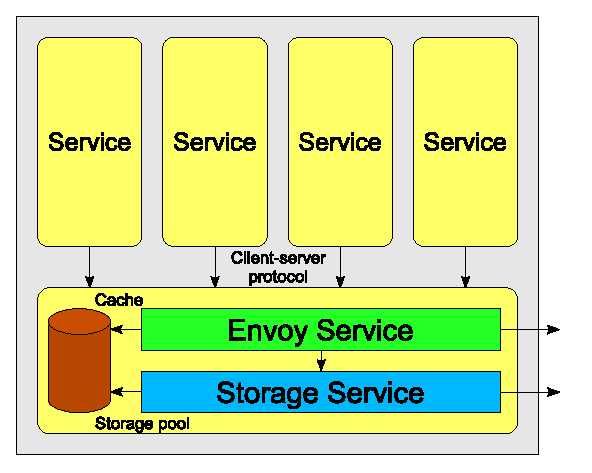
\includegraphics{figures/single-machine}
\caption{Each physical machine has a single administrative VM that hosts the Envoy services. This VM exports a network file system protocol to other service VMs running on the same machine.}
\label{fig:single-machine}
\end{figure}

The file system management processes join a cluster-wide service that is comprised of two primary layers, as illustrated in Figure~\ref{fig:layers}. Storage is managed by the lower level, which allows a small set of basic file operations on objects. All operations are stateless and the storage service makes no attempt to prevent or manage concurrent requests or to enforce any kind of security policy. Objects are extents of bytes with a small set of attributes.

On top of the storage service is the Envoy layer, which builds a hierarchical file system out of objects, coordinates access to files, provides authentication and access control services, manages caching, and exports a standard network file system interface for services to access.

\begin{figure}[tp]
\centering
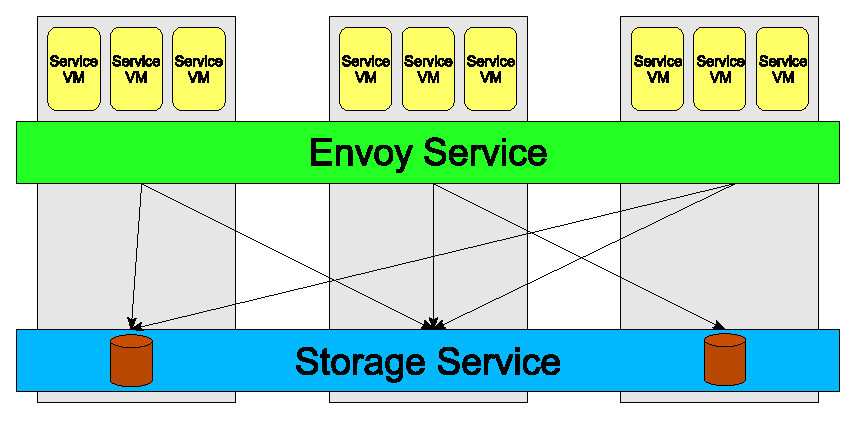
\includegraphics{figures/layers}
\caption{The Envoy services coordinate access to provide a single, coherent view of the distributed file system. It relies on the storage service, which provides a repository of objects referenced by unique identifiers.}
\label{fig:layers}
\end{figure}

In the remainder of this section I detail the functionality and requirements of these systems and consider the tradeoffs of various design decisions.

\subsection{Distribution}

Figure~\ref{fig:client-server} depicts a commonly-used storage arrangement using a series of dedicated file servers to handle the needs of many clients. This architecture is successfully used in many settings and, despite alternatives developed over the years, is still the dominant storage model in practical use.

\begin{figure}[tp]
\centering
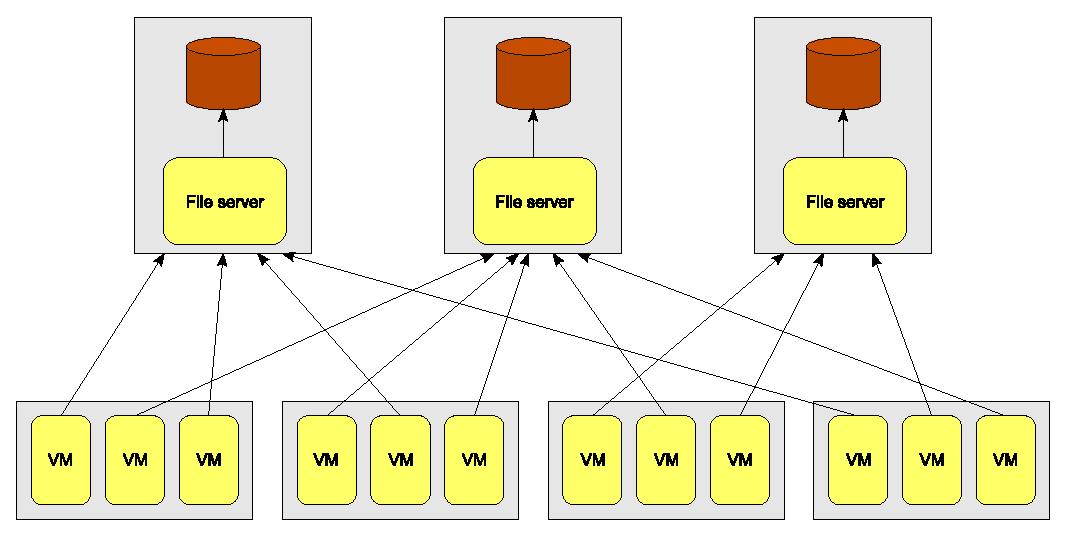
\includegraphics[width=100mm]{figures/client-server}
\caption{A popular storage solution for groups of clients involves a series of dedicated servers. Content on the servers is carefully managed to distributed storage demand and transaction load between the servers.}
\label{fig:client-server}
\end{figure}

The client-server model has obvious flaws when applied to clusters with many transient clients. Data placement decisions must balance space requirements and expected access rates in order to avoid overloading a particular server. Rebalancing---a disruptive and time consuming job---may be necessary in response to added clients, added servers, added disks, variations in client workload, and accumulation of data over time.

With the service cluster model, the problem is made even worse. To make efficient use of increasingly powerful hardware, each physical machine may host many services, each of which requires a boot image as well as access to the data relevant to its intended task. Single-purpose services may also be short lived or vary by time of data, making manual balancing impractical.

The client-server model has not endured as long as it has simply for lack of alternatives, however. It has many strengths that can inform the design of a more distributed architecture. With a single server managing shared data, concurrent access can be managed simply through explicit leases and cache invalidation, centralized caching with synchronous access, or through a lock manager. Whatever the mechanism for resolving conflicts, a centralized server is ideally suited to detecting and responding to concurrent requests because it is the point on the access graph at which all requests converge. The consistency of data that has reached the server is as good as its backing store.

The simplicity of a server is also a virtue. A failstop model for reliability can generally be assumed, backups are relatively straightforward, the server is typically dedicated to a single task or is shared with other trusted services, and the semantics are simple to define in terms of client behavior%
\footnote{NFS versions 2 and 3 have notoriously complicated consistency semantics, but this is almost entirely due to client policies. NFS server semantics are straightforward.}.

The chief faults of a centralized system are the introduction of a single point of failure and the inability to scale beyond the network and disk bandwidth that can be hosted by a single server. While these limits are unacceptable at large scales, they are quite reasonable for small groups of clients.

For clients that are sharing data, it is difficult to improve on a centralized server. For sufficiently overlapping data sets, any consistent model will degrade to something resembling a server during periods of contention because all interested clients will have to synchronize their access to the contended bits. A single arbitrator will ultimately oversee each bit of data, whether it is a traditional server, a lease-holding client, or a quorum of cooperating peers.

Sharing cache space is also a benefit of consolidated control of shared data. As the performance gap between disk access and memory access continues to grow, efficient use available cache space becomes increasingly important. Once again, a single centralized cache fails the scalability requirement, but a shared cache for a smaller set of clients with overlapping data needs provides attractive properties. Accessing a cache across a high-speed network is faster than accessing a local disk \cite{dahlin94b}, so in a cluster setting, organizing the aggregate cache around shared access patterns is more valuable than organizing it to localize access. Stated another way, the combined effective cache size of the entire cluster is greater when redundant entries are consolidated through sharing, and maximizing the combined cache size to avoid disk seek penalties is becoming more important than avoiding the network hops that arise from using a shared cache.

While a server cannot handle an unlimited number of clients, it can serve many clients under typical workloads. Scalability matters more at the level of the entire distributed system than when considering individual nodes. In the case of overlapping requests from different clients, a shared cache on a shared server will outperform a series of private servers, despite the overhead of network latency. Given that runtime contention is relatively rare \cite{kistler}, Envoy is designed to localize file ownership when there are no apparent conflicts, but to pick one participant to own files that are shared and act as a server to the others.

This principle of localizing control where possible, but reverting to a simple, well-understood client-server model when sharing is necessary is fundamental to Envoy. It leads to \emph{fate sharing} amoung clients with overlapping interests in the areas of performance, resource usage, and failure recovery. In each case, services with overlapping resource demands cooperate directly with each other and disinterested parties are not involved.

The overall distributed architecture of Envoy is modeled after human-administered systems using client-server file systems. Storage is distributed over a series of servers in an attempt to balance demand (the seperate storage layer handles balancing capacity), but where a human administrator is constrained by practical concerns to using relatively few, well-provisioned servers, an automated system can continue the process of server division and balancing to a much more fine-grained level. Entire images or parts of images that are used exclusively by a single service (or a group of services hosted on a single physical machine) are managed directly by the Envoy service on the same machine. Where sharing occurs, the client with the highest demand retains direct control and acts as a proxy for other clients accessing the same storage, thus sharing a cache and avoiding complicated coordination protocols.

\subsection{Storage layer}

The objective of the storage layer is to provide a simple, stateless interface for accessing objects. Redundancy to enhance availability and reliability and distribution to balance load is also handled by this part of the system. The storage layer is implemented in two parts, called the top and bottom halves.

The bottom half is implemented in the storage daemon hosted on each physical server. While the storage daemon instances form a collective pool of storage, they do not communicate directly with each other. At the local level, each storage manager is unaware of any global state, and responds blindly to incoming requests from the Envoy layer. Instances do not attempt to balance load, resolve conflicting requests, or create redundancy, nor do they monitor which object IDs they considered valid. Instead, they provide a thin, simple storage service for numbered objects with attributes.

To make these servers more useful, the top half of the storage layer is implemented in the Envoy daemon. It is responsible for mapping an object ID to the set of storage server instances that host the referent object. Combined with the persistent cache, the storage layer top half provides a simple procedural interface to the storage layer, where objects are named by unique IDs. The top half is responsible for creating and locating replicas, detecting and masking/recovering from failures, allocating new object IDs when needed, and reading and writing data and attributes.

Numerous strategies are available for distributing objects across the cluster. While I discuss some of them here, I only do so with the intent of demonstrating that an independent storage layer is viable and reasonable; many other object storage systems of varying levels of sophistication could be substituted for one I describe and other work has addresses object storage in more detail than I attempt here. The emphasis of this dissertation is on the Envoy layer as implemented on top of the object layer.

\subsection{Envoy layer}

The Envoy layer forms a file system from the objects provided by the storage layer, coordinating and caching access to the file hierarchy, and exporting a client-server protocol to services that act as clients of the file system.

A single instance of the Envoy service runs on each physical machine. The global name hierarchy is divided amoung participating instances in the cluster. When a given instance takes responsibility for some part of the namespace, it is said to \emph{own} a \emph{territory} covering the relevent subtree of the hierarchy. All operations within local territories are served locally and may be cached locally both in memory and in the persistent cache, which is reserved exclusively for territories local to the machine.

This partitioning of the global namespace and the resulting federation of constituent parts is what gives Envoy its name. When clients request operations that stray from the local territories, the requests are handed off to the Envoy on the appropriate machine. It follows that each instance must know not only the boundaries of its own territories, but how to find the Envoy for neighboring territories, i.e., those that can be reached by a single directory traversal (up or down) from a local territory.


\subsubsection{Data layout}

\subsection{Caching}
\subsubsection{Data paths for typical requests}

\section{Operations}
\subsection{File operations and state management}
\subsection{Forks and snapshots}
\subsection{Lease migration}
\subsection{Security}
\subsection{Deleting snapshots}

\section{Dynamic lease management}

What we really want is a dedicated guy running around setting up little servers near the interested clients and rearranging them as traffic stabalizes. A healthy dose of laziness may even be an asset---keep it simple and avoid thrashing.

\section{Recovery}

\section{Summary}
\chapter{The Envoy Prototype}

Even the simplest file systems involve complex interactions between numerous hardware and software components, and distributed file systems compound that complexity. While all modern designs tend to draw heavily on prior work, the particular combination of classic components and new innovations that make up a new system like Envoy can only be validated with empirical results.

I have implemented a prototype of Envoy to make testing possible and to permit a level of refinement in the design that is only possible with practical experience. This chapter first details the goals and parameters of the prototype, then discusses aspects of the implementation that shed further light on the design, expose its limitations, or show how implementation choices have shaped the prototype.

\section{Scope and design coverage}

\subsection{Goals of the prototype}

* Sanity check
* Test effects of runtime migration
* Check performance of machine-level caching vs. OS-level caching
* Check performance of shared access, remote vs. local

\subsection{Implementation shortcuts}

\subsubsection{Synchronization}

The prototype uses a simplified concurrency model based on a few assumptions. Concurrent transactions are permitted and executed on individual processor threads, but only one is allowed to execute at any given time. A global lock is held by the running thread, and is released whenever a network or disk operation is invoked. This simplifies shared-memory management considerably, and is justified on the assumption that the processing time for transactions is dominated by I/O latency.

\subsubsection{Caching}

Use the underlying OS to cache stuff. No need to reinvent the wheel here. Note that this makes good sense, it's not really a limitation. Set the size of the envoy service VM to control the cache size, take advantage of advances in the underlying OS, focus on the problem at hand.

\subsubsection{Garbage collection}

\section{The 9p protocol}

Clients access Envoy using a client-server file system protocol between the virtual machine of the client and that of the envoy service. While a custom protocol would offer the greatest flexibility, it would also make the implementation considerably more complicated and would have little value in demonstrating the viability of the design.

\subsection{Alternatives}

With Linux as the client operating system of choice, a few prominent options were available but ultimately rejected for the prototype.

\subsubsection{NFS version 3}

The NFS protocol is popular, simple, well-understood, and has a robust implementation. Most of the complexity is implemented in the client drivers, so servers can be quite simple. I also had experience with the protocol after implemented a stackable, copy-on-write file system (CoWNFS) for the XenoServers deployment project \cite{kotsovinos}.

For user mode servers generally and Envoy in particular, however, the stateless model of NFS complicates implementation. File handles assigned by the server and given to the client are expected to be immutable and always available (there are no explicit open and close operations), making it difficult to maintain pairings between active files and the envoy instances that own them. With transparent copy-on-write, these handles must either be cached indefinately or inherently tied to the name of the file. Changing territory boundaries makes caching impractical, and allowing for higher-level directories to be renamed makes the latter difficult to make robust.

Security under NFSv3 is based on Unix user and group IDs, which proves to be an inflexible mechanism when diverse clients become involved. The ID space must be shared between clients that share file systems, or the server must provide a mapping service to reconcile the differences. While not an insurmountable problem, this can get unnecessarily complicated when a client mounts multiple file system images, many clients share some images, and parts of those images are forked from standard base images.

The caching model of NFS is entirely under the control of the client driver, which generally sends frequent \texttt{stat} requests to check if its cache is still current. Write operations are generally asynchronous, however, and the lack of control would have defeated the cache coherency guarantees that Envoy seeks to achieve. Caching at the client level would also prevent consolidation of duplicate caches as the physical machine level, another of the aims of the Envoy design.

\subsubsection{NFS version 4}

The most recent update to NFS addresses many of these concerns by introducing a stateful model and using leases to manage client caching. These client delegations could work well with Envoy, allowing private files to be cached by the client and shared files to be held back and cached by the envoy. More flexible file handles and explicit state management also a better match. NFSv4 would be an attractive candidate for a future implementation, but at the time the Envoy prototype implementation was started, it was still relatively immature and the supporting tools were complicated to use and poorly documented.

\subsubsection{AFS}

The Andrew File System is another popular client-server system with a mature implementation. It employs persistent caching at the client, which is a poor fit for the Envoy model, and it is not intended as a general-purpose protocol for implementing custom servers. Adapting it to a system with very different semantics and basic assumptions would negate the benefits of using an establised protocol and implementation.

\subsubsection{FUSE}

The FUSE driver and tools support custom userspace file systems under Linux. The FUSE interface is modeled after the Linux VFS interface and exposes some of its complexity, but the main point against using FUSE for the Envoy prototype is that it is not a network-facing protocol. A userspace tool for the client would be required that would in turn connect to the envoy service across the virtual network device. Besides adding an unnecessary layer of indirection, this would complicate using Envoy as a root file system.

\subsubsection{Custom Envoy client driver}

Another possibility would be to implement a custom kernel driver for the Envoy client as well as the Envoy server. This would permit an exact between the expectations of the client and the semantics supported by the server. It would also permit optimizations precluded in standard drivers by the need to support a diverse range of servers.

Using a custom driver would have disadvantages, among them the need to divert time away from the server or to extend the total implementation time required. A custom driver would not be available in standard software distributions, either, requiring additional deployment effort for end users. Finally, a protocol would make evaluation more difficult by making it harder to isolate the costs of the Envoy deployment model from the costs of the protocol and client implementation. Being able to compare Envoy performance against other servers using the same client driver may penalize the overall performance, but it also allows a more detailed analysis of the results.

\subsubsection{9p}

The Envoy prototype is implemented using the 9p protocol from the Plan~9 operating system \cite{pike90,pike92}, which is specified in section 5 of the Plan~9 manual \cite{9man}. Plan~9 breaks from Unix semantics in many ways, so the Linux port of 9p has been extended to better support Unix semantics \cite{hensbergen}. The 9p protocol is intentionally simple. Individual connections are established for each user, and file ownership is tracked using user and group names, not numeric identifiers. The protocol includes no explicit support for client-side caching beyond the availability of file version tagging that could support NFS-style cache validation checks.

The 9p protocol is based around the thirteen messages listed in \prettyref{tab:9p-messages}. Authentication is achieved through an arbitrary sequence of reads and writes to a special file handle established with the \texttt{auth} message, and after the server is satisfied the client can follow-up by attaching to a specific point in the file hierarchy. Access to the rest of the hierarchy is through \texttt{walk} messages that move new or existing file handles through the namespace, and normal operations that can then access files and directories through the associated file handles.

\begin{table}[tp]
\begin{center}
\begin{tabular}{lp{8cm}}
\textbf{Message name} & \textbf{Description} \\
\texttt{version} & Initial handshake; establish message size limits. \\
\texttt{auth} & Authenticate a user to mount a specific path name. \\
\texttt{flush} & Cancel a pending request. \\
\texttt{attach} & Mount a specific path for a specific user. \\
\texttt{walk} & Navigate directories and/or clone a file handle. \\
\texttt{open} & Open a file or directory. \\
\texttt{create} & Create a file or directory. \\
\texttt{read} & Read bytes from a file or entries from a directory. \\
\texttt{write} & Write bytes to a file. \\
\texttt{clunk} & Release a file handle and close the file. \\
\texttt{remove} & Delete a file or empty directory. \\
\texttt{stat} & Read attributes for a file. \\
\texttt{wstat} & Change a file's attributes.
\end{tabular}
\end{center}
\caption{The messages in the 9p protocol. \texttt{version} and \texttt{auth} prepare a connection for an \texttt{attach} request, which establishes a single file handle. \texttt{walk} can clone or move existing file handles, giving access to the rest of the file tree. \texttt{flush} relates to an individual transaction, but all other messages operate relative to an active file handle.}
\label{tab:9p-messages}
\end{table}

\subsection{Mapping Envoy to 9p}

For basic file operations, an envoy acts like a 9p server to the client. The service connects over a virtual network device that connects the service VM to the VM hosting the envoy service. While the prototype uses a standard TCP connection for communicating, 9p supports any transport layer and could use an interface for virtual machine environments that swaps memory pages between VMs instead of copying data through the standard network protocol stack. While this has not yet been implemented for 9p servers, it is a potential optimization that could reduce the additional cost of retrieving data from the machine-level cache over retrieving it from an OS-level cache in an individual VM.

\subsubsection{File handles and state management}

When a file is owned remotely, the local envoy acts as a proxy server and forwards requests to the appropriate envoy. Like client connections, forwarded transactions are tracked relative to file handles owned by specific users.

File handles are tracked by small positive integers, which are unique in the context of a specific connection. When acting as proxies, envoys map client identifiers to \emph{remote identifiers}, which are unique for a given envoy instance. This allows envoys to combine all requests from their constituent servives when contacting a remote envoy, effectively making the envoy act like a single client. By making the identifiers unique for all outgoing requests from the envoy instead of for each local-remote envoy pair, no remapping is required when file handles migrate from one remote envoy to another during territory realignments.

\subsubsection{Security}

\subsubsection{Caching}

\section{Storage service}

The storage service implements the bottom half of the storage layer, which is essentially an independent, stateless object server. Each server that contributes storage space runs a single instance of the storage service to export an object-level interface.

The storage layer is underspecified. It is an essential part of a complete Envoy implementation, but object management systems are not the subject of this dissertation, which instead focuses on building a complete distributed file system above an object-storage layer. The artifact described here is a stub, offering enough support to complete and test the file system build above it, but not enough for a production setup.

The remainder of this section describes the protocol used by the storage servers, and discusses the implementation of the object store.

\subsection{Protocol}

The storage server protocol is implemented as an extension of the 9p protocol. It uses the same RPC mechanism and shares the same hand-shaking messages. Like 9p, it does not define an authentication protocol, but instead provides a framework for implementations to exchange credentials. In its intended setting, authentication could also be based solely on IP addresses, since the entire network is controlled and virtual machines can easily be prevented from spoofing their addresses.

\prettyref{tab:storage-messages} lists the messages unique to the storage server. The \texttt{reserver} message lets an envoy request a range of previously unallocated object IDs for its later use. Since storage servers do not communicate with each other directly, envoys must agree to consult a single storage server in a particular replica group, i.e., amoung those servers storing a given range of object IDs, to prevent overlapping allocations.

\begin{table}[tp]
\begin{center}
\begin{tabular}{lp{8cm}}
\textbf{Message name} & \textbf{Description} \\
\texttt{reserve} & Claim a range of unallocated object IDs. \\
\texttt{create} & Create a new object. \\
\texttt{clone} & Copy an existing object, set copy-on-write flags for directories. \\
\texttt{read} & Read a byte range from an object. \\
\texttt{write} & Write a byte range to an object. \\
\texttt{stat} & Query an object's attributes. \\
\texttt{wstat} & Modify an object's attributes. \\
\texttt{delete} & Remove an object. \\
\end{tabular}
\end{center}
\caption{The messages in the storage service protocol. \texttt{reserve} returns a range of object IDs previously unallocated by the same storage server. \texttt{clone} copies an object, and if it is a directory it also sets the copy-on-write flag for all entries in the new copy. All operations except \texttt{reserve} are stateless, requiring an object ID as well as operation-specific parameters.}
\label{tab:storage-messages}
\end{table}

In a centrally-controlled cluster, assigning ranges of object IDs to storage servers and picking master replicas is a job best accomplished by a centralized, possibly replicated server. Likewise, coordinating bulk transfers of objects between servers to accomodate new nodes or compensate for failed machines is much easier to manage from a single location than to manage using a distributed protocol. Such tasks would be light work even when controlling many machines, because the events that require coordination occur infrequently. Unlike peer-to-peer systems, managed clusters can trust individual nodes and avoid distributing tasks that are better handled by centralized services.

The \emph{clone} operation, which copies an object from one given ID to another, is the only procedure that differentiates regular file objects from directory objects. When the attributes indicate that an object being cloned is a directory, the storage server will expect it to follow a particular format (described in \prettyref{sec:directory-format}) and will set the copy-on-write flags within each block as it makes the copy. It is not essential that this functionality be part of the storage service, indeed the clone operation itself could be implemented in terms of the other procedures. It is merely a performance optimization to avoid extra network round trips when possible. When a copy is required from one storage server to another (when the envoy is directed to create new objects on a different server than an existing object) a more conventional sequence of reads and writes must occur.

The other operations are straightforward, though it is worth noting that they differ from the related 9p operations in an important way: they require an object ID as a parameter instead of an active file handle. Envoys can make and break connections to storage servers as needed without losing any state. A pool of connections to frequently used storage servers is an obvious optimization, but is not strictly necessary.

\subsection{Implementation}

The storage service is implemented as part of the same executable as the envoy service. The two must be run as seperate processes even on the same virtual machine, but since they share an executable image they can also run from the same shared memory blocks. Combining them is convenient because they share a lot of code.

The protocols for 9p clients, the storage service, and the envoy service are implemented as one single set of messages, only some of which are considered valid for each connection type. This allows shared code for network management, concurrent message dispatch, and numerous lower-level libraries. The code for storing objects on disk is also used by the envoy service for managing the persistent cache.

\subsubsection{Disk layout}

Each object is stored as a file in a normal Linux file system. Objects are stored in a hierarchy of directories, arranged to create a radix tree indexed by the object ID. In this scheme, a 64 bit object ID is broken into a series of smaller bit sequences, each of which (as a hexadecimal string) names a directory in the path to the object.

The least-significant bits of the object ID are used in constructing the file name. Each node name in the tree need only identify the few bits that distinguish the branch of which it is the root---the entire path taken together identifies the full ID of the object.

The number of bits partitioned into each directory level is significant. It is chosen to be the largest value $n$ such that a directory with $2^n$ entries named by hexadecimal strings encoding $n$ bits each will fit in a single disk block on the underlying file system. This structure turns the file system into a crude radix tree with block-sized nodes, and uses the OS buffer cache for the indexing structure in place of a custom cache.

The bit-splitting process starts with the least-significant bits and proceeds to the most-significant bits, ensuring that if any level of the index has a smaller fan-out factor than any other, it will be the root. This is for two reasons: squandering space in a single root block is preferable to wasting an equivalent factor of space in every leaf node, and less critically, changing the number of bits in the object ID for an existing object store can be done by manipulating a few entries at the root and leaving all other nodes untouched.

\subsubsection{Directories and metadata}

The number of bits from the object ID stored in the file name at the leaf node is also different from the higher-level directory nodes. While some of the object attribute fields are provided by the backing file system, others fields are stored as strings in the file name itself. File names are of fixed length, and encode both the bits that distinguish the object from its immediate neighbors and object attributes that are not easily stored as file attributes.

As with the interior nodes of the radix tree, the number of files in a leaf directory is chosen to keep the directory in a single disk block. When the system looks for an object, it reads the entire directory that will hold that object and caches the results. This gives it the precise file name for the object (along with the metadata stored in that name) and also primes the buffer cache with the directory block, so when the object file itself is accessed it will be located through the cached directory. In this way, extra attributes can be accessed from the file names without incurring extra disk seeks.

The attributes stored in the file names are the file mode and names of the user and group that own the file. The mode (including access permissions and the file type) cannot be freely read from and written to in its entirety in normal file systems, so encoding a device or a directory as a normal file requires storing the type somewhere else. While access permissions could be stored in the standard mode attribute, they would be honored by the underlying file system and would prevent unfettered access by the storage manager. User and group names in Envoy are stored symbolically, while most Linux file systems store them as numeric IDs, and again the file system's recognition of their semantic meaning would interfere with the storage manager. Storing any of these fields as a prefix to the actual file contents would violate block alignment assumptions that many clients make about file data, so an external mechanism was desirable.

While access to files in the object store is stateless, the access patterns of normal file system use are applicable to objects. Because of the persistent cache, entire files are often read in sequence, a common pattern for client operations as well. The storage service caches open handles to the most recently accessed files, both to avoid having to re-open them on each request and to avoid giving the backing file system a false hint that the file is no longer needed. Open file handles are kept on a strict LRU basis, as are the cached lists of file names in leaf-node directories mentioned above.

\subsubsection{Caching}

Envoy considers a write request finished when it is in the memory of the storage servers for all replicas. While this opens a window during which the data could be lost by a system crash, it is unlikely that multiple replicas would crash during the same window (assuming that nodes in the cluster are sufficiently isolated from each other). The storage server immediately passes all requests through to the underlying file system, and relies on the OS buffer cache to implement delayed writes. This is the simplest approach to implementation (use someone else's) but is also a sensible choice. Little would be gained by a custom solution, and this approach takes advantage of continuing improvements in the operating system. Indeed, taking advantage of continuing improvements in commodity hardware and software is one of the primary motivations for the this work.

\subsection{Limitations}

The storage server implementation is meant to be as simple as possible while still supporting realistic workloads. With the intention that a production design would take advantage of other work in object storage systems, the prototype neglects several important characteristics of a complete system:

\begin{itemize}
\item Security: while the mechanism for authenticating envoys at connection time exists, no authentication is attempted in the prototype. From a performance standpoint, a challenge-response scheme or something similar would be a startup cost that is ignored in the prototype. It would be largely hidden by even a moderately-sized connection pool, but it would be present. In a controlled environment like a service cluster, a scheme based on IP addresses would be faster, simpler, and just as secure in practice. IP addresses could be assigned according to the role of the owner, so traffic from client VMs could be easily identified by all, and the VM hosting envoy and storage services could employ a firewall to prevent storage servers from ever seeing client requests.

\item Replica groups: the top half of the storage layer, i.e., the part that maps object IDs to storage servers, is essentially absent from the prototype. For any large deployment, a suitable disbursement of objects across storage servers is essential. Different degrees of failure protection may be desirable as well, with increased replication being available to clients at a premium cost.

\item Redistribution: when nodes are added or removed from the cluster, objects must be moved and copied to maintain a suitable replication factor. While I have stated that this could be controlled by a centralized service, no mechanism currently exists for copying directly between storage servers (other than systems such as \texttt{rsync} that bypass the storage service and go directly to its object store). These capabilities are critical to a system that will change over time, which is a basic characteristic of any realistic cluster deployment.

\item Failure: recovery of a crashed envoy node is addressed in \prettyref{sec:envoy-recovery}, but recovery of a failed storage node is an equally important problem. While redundancy allows the envoy layer to continue serving files, changes made during the downtime must be propogated to the restored node to ensure consistency, and nodes that do not recover must be replaced or their stored objects redistributed.
\end{itemize}

Despite the absense of these essential features, the storage prototype does implement replicated storage with all the characteristics necessary to support the envoy layer. As that is sufficient for the stated purposes of this dissertation, the prototype is also considered sufficient.

\section{Envoy service}

The envoy service runs on each node to form a single, distributed service across the cluster. It exports a view of the global namespace by acting as a 9p server to VM clients running on the same physical machine. Each instance assumes responsibility for specific territories, or subsets of the namespace. The name \emph{envoy} comes into play in two respects: it negotiates contact between local clients and the larger system, and acts as representative for its local territories to other nodes in the cluster and their constituent clients.

This section starts by describing the protocol used for inter-envoy communication, and then proceeds to discuss some internals in the envoy implementation. This includes details about basic file operations and navigation between envoy instances, the copy-on-write mechanism behind the fork and snapshot operations, and the coordination of state during territory boundary realignment.

For operations that require the synchronous cooperation of multiple envoy instances, dependency cycles and deadlock become a concern. To minimize these issues, Envoy is designed with a top-down locking protocol where synchronous operations only directly involve immediate neighbors in the tree of territories, and owners of parent territories always initiate and coordinate transactions with those lower in the tree. While operations with wide-ranging impact may require communicating with every node in the cluster, they never require a cycle in the connectivity graph and are not prone to distributed deadlock.

\subsection{Protocol}

As with the storage service, the envoy services protocol is implemented as a series of extensions to the 9p protocol. The integration is closer at the envoy level, however, as forwarded transactions from remote clients use the standard 9p messages when appropriate, depending on the extensions listed in \prettyref{tab:envoy-messages} mainly to implement territory management and handle operations that straddle territory boundaries.

\begin{table}[tp]
\begin{center}
\begin{tabular}{lp{8cm}}
\textbf{Message name} & \textbf{Description} \\
\texttt{snapshot} & Take a snapshot of a territory. \\
\texttt{nominate} & Request that the parent transfer control of a territory. \\
\texttt{grant} & Give the target control of a territory. \\
\texttt{revoke} & Reclaim control of a territory. \\
\texttt{migrate} & Inform an envoy of file handles that have moved. \\
\texttt{walkremote} & Change directories across a territory boundary. \\
\texttt{statremote} & Query file attributes across a territory boundary. \\
\texttt{closefid} & Release an old file handle after it has walked to a new host. \\
\texttt{renametree} & Inform descendents of a directory that has been renamed.
\end{tabular}
\end{center}
\caption{The messages in the envoy service protocol. The first five support the major state management operations, while the remainder handle cases where an operation affects multiple territories.}
\label{tab:envoy-messages}
\end{table}

Envoys establish connections with each other only when they need to, specifically when they have neighboring territories or when transactions from one envoy's clients involve a territory owned by another envoy. Neighboring territories always form a tree structure, with one territory in every pairing (and by extension its envoy) being considered the parent of the other.

New connections between envoys must be authenticated in a way similar to connections between envoys and storage servers. The handshake messages from 9p are used, with the protocol string in the \texttt{version} message identifying the connection as one between envoys so that the appropriate range of messages will be understood. Authentication can proceed through an exchange of credentials, or the controlled environment of the service cluster can be exploited and network addresses can be used to identify authorized service hosts.

9p messages from \prettyref{tab:9p-messages} are all considered valid coming from other envoys, with the exception of the \texttt{walk} and \texttt{attach} messages, which are replaced by an augmented version called \texttt{remotewalk} that accomodates territory boundary changes. Transactions still proceed in relation to normal file handles, with the further restriction that an envoy will never forward requests as a proxy for another envoy, only for clients.

\subsection{Data structures}

Unlike the stateless storage servers, envoy instances must track two main classes of state related to the two main roles an envoy assumes, namely those of 9p file server and territory owner.

\subsubsection{Territories and claims}

\begin{figure}[tp]
\centering
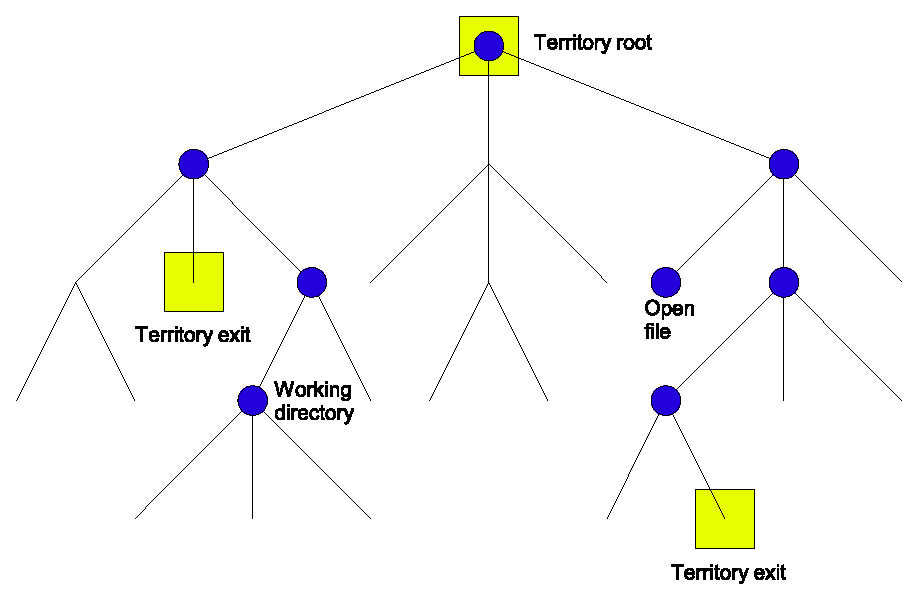
\includegraphics[width=100mm]{figures/territory-claims}
\caption{Territories are trees, and their boundaries (yellow squares) are defined by the root pathname and the exits, which point to child territories owned by remote envoys. Claims (blue circles) represent individual storage objects, and within a territory they form a tree covering a subset of the territory, with leaves at each territory exit and active file or directory.}
\label{fig:territory-claims}
\end{figure}

An envoy may own zero or more territories, each of which is a branch of the global file tree, possibly with exits to child territories owned by other envoys as depicted in \prettyref{fig:territory-claims}. When the territory is given to the envoy through a \texttt{grant} message, it is also given the object ID that currently backs the root directory or file (a territory can be a single file) and a flag indicating if the object is writable. A territory may cover a snapshot image, in which case all objects are read-only. The root of the territory is never flagged as copy-on-write, so thaw operations (described in \prettyref{sec:freeze-thaw}) can always operate locally.

Overlaid on the file tree within a territory is another tree of \emph{claims}, or references to storage layer objects. Claims are maintained for all file handles, territory exits (actually the immediate parent directories of exits), and the path from any other claim back to the root of the territory. It is possible for multiple claims to exist for a single storage object, but only when the claims are all read-only or copy-on-write, and thus the associated objects are read-only. In this case, coordination for accessing the object is not necessary, and the file cache will recognize them as the same object to avoid duplication.

\subsubsection{File handles}

\begin{figure}[tp]
\centering
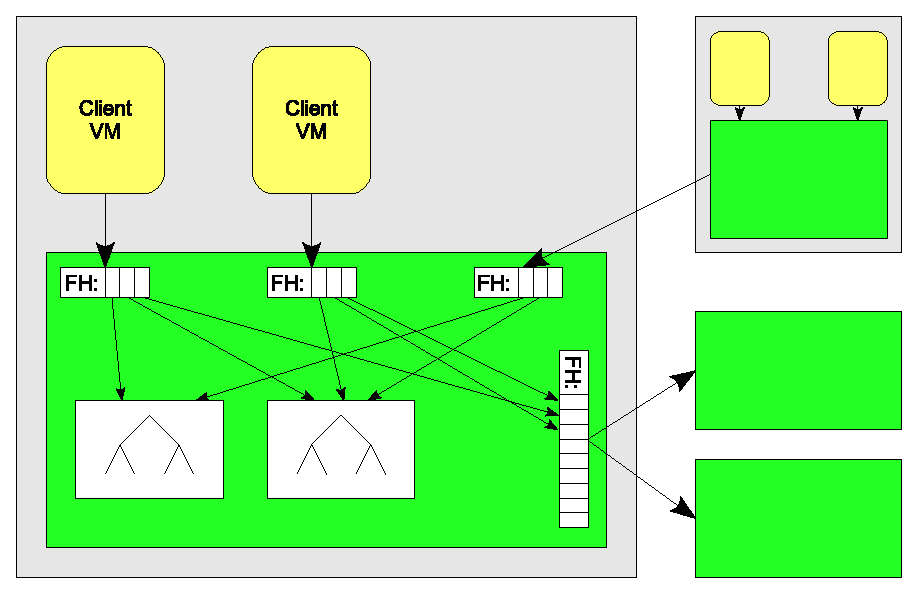
\includegraphics[width=100mm]{figures/file-handles}
\caption{File handles for incoming connections are grouped and distinguished by the source, be it a client VM or a remote envoy. Each handle is tied to a specific claim in a local territory. Client handles may also be forwarded to a remote envoy, in which case it is assigned an entry from the envoy's single remote file handle pool.}
\label{fig:file-handles}
\end{figure}

File handles in 9p are identified by small positive integers picked by the client, so the envoy interprets them in relation to the incoming connection. This gives each client a seperate namespace, preventing confusion when resolving file handle IDs to file handles. All clients represented by a remote envoy are combined into a single ID space, so the envoy receiving the requests treats the entire envoy and all the clients is represents as a single client, as illustrated in \prettyref{fig:file-handles}. Since the user credentials are associated with individual file handles, this does not confuse security handling. Envoys-as-clients are not quite like regular clients, as their file handles are never re-forwarded; instead, when a file handle moves to a new territory the handle is sent back to the original envoy, which can forward it directly to the appropriate target.

When forwarding client requests for remote territories, the envoy remaps the client ID to an envoy-specific remote ID. A single pool of remote IDs serves all outgoing connections, regardless of their targets, which simplifies territory migration as described in \prettyref{sec:migrating-state}. The envoy also maintains a local file handle stub for remote files, which is kept up-to-date by peeking at the requests and responses for remote operations. In this way, state for local clients is lost when an envoy fails, but state for remote envoys and their clients is preserved and can be used to recover from the failure.

\subsubsection{Persistent cache}

The persistent cache is the other major source of state in an envoy. On-disk objects are managed using the same code as the storage service uses for managing the object store, with the same disk structure and the same reliance on the underlying file system for in-memory caching.

The significant difference between the cache that an envoy maintains and the object store tended by a storage server is that the envoy must determine which objects are properly synchronized with the storage layer. Validating an unknown entry (one found in the persistent store but whose status is unknown) can be accomplished with a simple metadata comparison, so it is worthwhile keeping old objects even when the envoy has ceded the territory that referenced them, as it may eventually come back. Objects can be cleared when deleted, or based on a least-recently-used strategy. Once an object has been validated in the context of a territory that owns the object, it's validity need not be refreshed until the object has left local control.

\subsection{Freezing and thawing}\label{sec:freeze-thaw}

Synchronization at the object level is governed by an important invariant: an object in the system may be referred to by exactly one name in the hierarchical namespace, or it must be read-only. The storage layer makes no attempt to detect or enforce the read-only case, so it is left to the envoy layer to ensure that this invariant is preserved. To make this straightforward, objects can transition from being writable to read-only, but they can never go back. Note that this refers only to objects in the storage layer, not to the access control of file system objects.

The same invariant makes cache management simple: the envoy that owns a given territory can cache it without any invalidation concerns, and read-only objects can be safely cached at any number of envoy nodes without fear of interference. Objects in the cache become invalid only when a territory boundary changes. Objects that are part of ceded territory are not explicitly flushed from the cache; keeping them active helps in two cases: a read-only object may still be referenced by another name in a local territory, and the cache entry (in-memory or on-disk) may still be useful if a file backed by that object is later returned to local control. In the latter case the object must be verified to match the version in the storage layer, but this can be done with a lightweight metadata comparison.

The single mutable/multiple immutable dichotomy in the storage layer is tracked in the envoy layer through the copy-on-write flag in directory entries. The immutable property is not directly assigned to objects, but instead is imbued by the link from directory to file object. Furthermore, when the immutable object is itself a directory, the property is applied recursively to all of its children, overriding the individual copy-on-write flag in the link to each child. To be regarded as mutable, an object must be reachable by a path from the root of the global namespace to the directory entry linking to the object without traversing any copy-on-write flags that are set.

One immediate consequence of this is that taking a read-only snapshot of a directory and its descendents requires only setting the copy-on-write flag in the link to it, an operation known as \emph{freezing}. Once a directory or file is frozen, the storage layer objects that back the branch rooted at that point are considered immutable. To simplify bookkeeping, this operation is only performed from the root of client images when a snapshot operation is requested. The benefits gained from this restriction and an exception to it are discussed in \prettyref{sec:hard-links}.

The complementary operation is called \emph{thawing}. While the freeze operation works at the root of a subtree and affects it in its entirety, thawing aims to leave as small a footprint as possible; it is always performed with the goal of modifying a particular file. To thaw a file, the owning envoy starts walking up the line of its ancestors until it finds one that is already thawed. As the root of the namespace cannot be frozen (one can consider it as having a single, implicit link from the envoy service itself, but there is no mechanism provided to set the copy-on-write flag on this implicit link), this search is guaranteed to succeed. From there the envoy walks back to the target file, \emph{cloning} intermediate directories as it goes. In addition to making a copy of the directory as its name implies, cloning sets the copy-on-write flag of every directory entry in the copy, effectively transferring the copy-on-write property from the single link leading into the directory to all the links leading out of the directory. The implicit property that each child inherited becomes explicit after being passed down a generation. After thawing each directory for mutability, the parent is updated to reflect both the new object ID and the cleared flag. Eventually the intended target itself (be it file or directory) is cloned, its immediate parent link updated, and the file is fully thawed.

Thawing resembles the procedure for modifying a value in a tree in a functional language. In addition to changing the value itself, the path from that item to the root of the tree must be copied if the item is to be reachable from the root. In the thawing operation, it is only the root of the immutable subtree in which the item resides that must be copied. While the analagous procedure in a functional language copies everything exactly except for the path being changed, the thaw operation must clear the copy-on-write flag as it goes, and thus must push it down from parent link to sibling links at each level in order to preserve the immutable status of the unaffected branches.

The prototype clones an entire object, but it could be optimized to store deltas or otherwise compress changes, especially in directories and other metadata \cite{soules}.

\subsection{Read operations}

Most basic file and directory operations have a straightforward implementation. The need to cross territory boundaries makes some more complex, however, as they must coordinate with remote envoys to complete.

\subsubsection{Reading files and attributes}

The most straightforward operations are \texttt{read} and \texttt{stat}, which read the data and metadata of files, respectively. These requests can be filled using the data paths described in \prettyref{sec:data-paths-read}. The only complication involved is handling the \texttt{atime} attributed, which tracks the last time the data from a file was accessed by a \texttt{read} or \texttt{write} operation. Read operations always proceed through a single envoy, so this attribute can be tracked accurately: the envoy can send a message with the timestamp (to ensure that it is consistently applied to all replicas, even if all clocks are not in sync or network latencies between the different storage servers vary) to all replicas in the storage layer which can then update the attribute.

The intended meaning of the \texttt{atime} attribute becomes obscured when applied to frozen files, however. Since attributes are part of the object, akin to \texttt{inodes} in traditional Unix file systems, changing the attribute will affect all files that are backed by that same object. Those instances may be in read-only snapshots of the same file system image, or in common files available in an unrelated file system image. In the former case, the read-only property of the snapshot is broken, and in the latter case the isolation of the two images is compromized. Updating the \texttt{atime} attribute would give an unrelated client using the same prepackaged file system image the ability to losely track file accesses, which could represent a security risk.

Accurately tracking the \texttt{atime} attribute is problematic with frozen files, and if it is only updated on some files (which may change over time as successive snapshots are taken), it is too unreliable to be useful. It also generates network and disk traffic for every read, even those that can be satisfied from the cache. For these reason, the \texttt{atime} attribute is present in Envoy for compatibility, but it effectively mirrors the modified time attribute.

\subsubsection{Reading from directories}\label{sec:walk-cache}

Reading from directories introduces two complications. The first---that successive \texttt{readdir} requests require state that must be transmitted from the client each time or transferred to another envoy when territories are realigned---is just an implementation issue. The second---that a directory may span multiple territories---requires the cooperation of all affected envoys. The list of contents for a single directory is considered an atomic unit when drawing territory boundaries, but the files and directories named may be remote. If the client-server protocol used to export the file system to a service only requests names, then the implementation footprint resembles that of file reads. If the response includes attributes as well---as with 9p---additional requests must be forwarded to the respective envoys for all files that are across a boundary in order to ensure consistent results. These requests are sent directly by the owning envoy, so if the client is remote, \texttt{readdir} may require the cooperation of three or more envoys to complete a single request. When gathering file attributes, the envoy that owns the directory sends requests directly to the file owners, resulting in a star topology with the directory owner as the central node. An additional link from the client's envoy is necessary if the directory is remotely owned.

Multi-step directory navigation can also create a star pattern of requests, but they always center around the client's local envoy. Navigating down a series of directories---an operation called \texttt{walk} in 9p---may involve crossing a territory boundary at each step in the extreme case. Because an envoy confines itself to knowledge of its local territories and their immediate boundaries, it cannot always predict the endpoint envoy for a navigation. Even if it could, intermediate steps must always be taken to allow permission checking at each level. When a remote territory must be consulted, the client's envoy forwards all remaining steps in the \texttt{walk} to the remote owner, which proceeds as far as it can with the navigation. It may return one of three results: if the result is successfully completed, the two envoys store any state necessary to handle future requests; if the result is a failure, an appropriate error code is returned; if the navigation reaches another territory boundary, the partial result comes back along with a pointer to the envoy that must be consulted to continue the navigation. The client's envoy then repeats the procedure with the remaining navigation steps.

Because these operations are all asynchronous, and because the navigated directories may be owned by remote envoys that are not even neighbors to the client's envoy, \texttt{walk} may encounter transient failures. Between the time that one remote envoy returns instructions for forwarding the remainder of a request, the target territory may migrate to a new owner and the request will fail. Because the envoy that sent the forwarding instructions was an immediate neighbor of the target, its information must have been correct at the time, and careful coordination can ensure that by the time the target bounces the request back with a failure notice, the referrer knows of the change to its immediate neighborhood. The solution is simply to restart the request from the beginning, which will also correct the client's envoy for the cases of a directory being deleted or renamed.

Generally, having territory boundaries closely aligned with demand benefits everyone, but if multi-step directory navigations are frequent, their performance will be hurt by frequent boundary crossing. Caching \texttt{walk} results can be done safely with a few precautions. First note that a navigation that succeeds one time and fails another implies one of three things: one of the steps was deleted or renamed, permissions changed somewhere, or a different user requested the navigation. The prototype caches \texttt{walk} results keyed by the path traversed and the user that requested it. With the assumption that directory renames and permission changes are uncommon (particularly across boundaries determined by locality of reference---I expect these changes to be most common in a region being actively modified by a single player, not in higher-level directories whose descendents are in active use by different clients), envoys broadcast notification of such changes down the hierarchy when they occur, invalidating cached navigation results. The notification of permission changes is treated as a special case of directory renaming for cache invalidation purposes, as discussed in \prettyref{sec:rename-operation}.

Attributes at the endpoint of the navigation are always confirmed directly with the owner, as are all of the final steps that occurred on territory owned by that same envoy. With a hot cache, multi-step directory navigations are satisfied from the cache of the client's envoy and a single step to the envoy hosting the target of the navigation.

\subsection{Write operations}

\subsubsection{Writing data and attributes}

Like the corresponding read operations, writes to files and changes to file metadata are largely a matter of directing the request to the appropriate envoy. The first change to a file since a snapshot or fork will first require the file to be thawed, but subsequent changes can be made directly to the local cache entries and propogated to all replicas in the storage layer. As discussed in \prettyref{sec:data-paths-write}, changes are considered complete when they have been received by all storage servers, but not necessarily commited to stable storage.

To ensure consistent time stamps, the modification time is determined by the envoy that owns the file and transmitted to the storage layer along with the data being written. While the clocks of machines within a cluster can be synchronized within reasonable bounds, network latencies and variations in storage server load levels would make it difficult to rely on strict synchronization for consistent timestamps. The envoy is a natural location for deciding on the canonical time for its territories.

Thawing a file requires walking back in the file tree until an already-thawed directory is found. To bound the complexity of this procedure and to avoid deadlocks, the root of every local territory is always thawed unless it is part of a read-only snapshot image. While thawing may require cloning multiple levels of the directory hierarchy, this confines the direct impact to a single envoy. It also preserves the top-down rule for synchronous inter-envoy operations by preventing an envoy from demanding a bilateral change from its parent in the tree of territory ownership.

\subsubsection{Deleting files}

The \texttt{inode}-like disconnect between directories and the files they name means that one envoy may own a territory consisting of a single file, while another envoy owns the directory containing that file. Most operations involve either the file itself or the directory, but not both, so it is obvious which envoy should serve the request. Removing a file or directory is a case where the possibility of divided ownership complicates the implementation.

Deleting a file affects both envoys in this case, but the operation needs to appear atomic to clients. The normal rule in Envoy is that the parent should drive bilateral operations, meaning in this case that the owner of the directory should coordinate the removal with the owner of the file. This is a mismatch with 9p, where removal is an operation initiated on a file, not on the directory that contains it.

A higher-level consideration ultimately drives the design of the delete operation, however. Removal can only succeed on files or empty directories, so an envoy that owns the target of a successful delete will have nothing left to own afterward. Instead of trying to atomically coordinate a multi-step the operation between two envoys, the parent instead revokes ownership of the child from its envoy and reclaims it before proceeding.

Since 9p initiates removal with the file to be deleted and not its containing directory, this requires a minor slight-of-hand to maintain the top-down coordination rule. A \texttt{nominate} request is sent from the file's envoy to the that of the parent directory, requesting that it reclaim the removal target. Since \texttt{nominate} operations are implemented strictly in terms of names (not 9p file handles) this request cannot trigger a deadlock, and the remove transaction running on the child envoy effectively becomes a passive observer while control of the territory is transferred. After the transfer is complete, the envoy aborts the transaction and starts it over. Since the file is no longer local, the envoy will either forward the request (if it happens to be the client's local envoy) or reject it, forcing the client's envoy to redirect it to the new owner. \texttt{nominate} requests do not return until all state has been transferred, so the restarted transaction can proceed immediately.

Deletes happen in four basic steps. The first checks that the file is a suitable candidate for deletion, namely that it is a file or an empty directory. The second verifies that the client has permission to remove it from the parent directory, and the third actually removes it. In the case where the territory ownership must change, the envoy owning the file can complete the first step, but it does not know if the second step will succeed and blindly proceeds to initiate the transfer of control. This could cause unnecesary activity if the permission check fails, but in practice the Linux driver used in the prototype does an explicit check before making the delete request, so the possibility of failure is remote: it would indicate an uncommon race condition and does not compromise the correctness of the operation even then.

The fourth step in deleting a file is to actually delete the object that backs it and reclaim the storage space. This is simple enough to do, but deciding when to do it is slightly more complicated. An object can only be deleted when no more names link to it, and to support Unix semantics it should also be preserved until all clients accessing it have closed the file. The former case is easy to detect: if the link to the file was marked as copy-on-write, it shares a link with at least one snapshot and should not be removed. Otherwise, it was created or cloned in the current image since the most recent snapshot and can be safely removed.

To support familiar Unix semantics, the envoy instance strips waits until all file handles are closed before deleting the file. 9p is stateful, so this is straightforward, but it does create a few corner cases that must be dealt with. A new file with the same name could be created, so the envoy cannot continue to track the object by its former name. Without a name the file does not belong to any territory, so it becomes an orphan. Opening a file and deleting it is often done to provide a temporary scratch file that will delete itself if the process dies, but it may still be long-lived. The envoy must still be prepared to thaw it if it was frozen at delete time, migrate it to another envoy in response to demand or to the owning envoy shutting down, and delete the storage layer object even in the event of a failure. The prototype does not address all of these issues, but it does support arbitrary use of the file until the last file handle is closed, at which point the object is deleted from the storage layer if appropriate.

\subsubsection{Renaming files}\label{sec:rename-operation}

Renaming a file exposes the same coordination issues as deleting a file. In 9p a rename request is part of a \texttt{wstat} request, which treats the file name as a property of the file object rather than of the directory that contains it. With rename the issue is even worse than with delete, because up to three objects and three envoys may be involved: one owning the directory, one owning the file to be renamed, and the third owning an old file with the target name that will be implicitly deleted when the rename completes. To further complicate the issue, Unix programs assume that rename-with-delete will complete atomically. Note that the original 9p protocol does not support this (it calls for a failure if the target name is already in use) but the Linux implementation does support this arrangement, and many clients demand it.

As with delete, the prototype simplifies the problem by consolidating ownership of all participanting objects onto a single envoy before making any changes. Unlike the delete case, the renamed file exists afterward and may be a non-empty directory. If it was owned by a different envoy before, that envoy probably drives most of the traffic to it and annexing it into the parent territory may be a poor move for matching ownership with usage. One solution would be to transfer control back to the original owner after the rename completes. It would have to revalidate some cache entries, but they would still be mostly unchanged, and even the in-memory cache would still be usable after a single metadata check on each file. A second possibility would be to engineer a distributed version of rename for these cases, driven by the parent (as with all synchronous operations) and handling transient failures appropriately. A third approach (the simplest and the one taken by the prototype) is to assume that such renames are rare and do nothing. Correct behavior is still maintained, and eventually traffic patterns will force the owner to cede the territory once again if appropriate.

Renames of directories present another difficulty that cannot be safely ignored. Territory boundaries are all managed using directory and file names, so renaming a directory that is ancestor to other territories throws management state out of sync. On the assumption that renaming high-level directories is relatively rare, the prototype handles them by propogating rename events from parent territory to child and from owner envoy to client envoy when they happen, rather than trying to assign immutable aliases for directories or some other similar scheme. Minor overhead in the rare case is usually preferable to complexity in every case.

In addition to updating territory and file handle names, these tree-traversing rename messages flush the walk cache described in \prettyref{sec:walk-cache}.  While a more fine-grained invalidation could be implemented, in practice an occasional flush has very little affect on performance, and it offers a mechanism for solving another problem. As a special case, this message can be used to rename a directory to the same name, forcing a recursive flush of the walk cache but not changing anything else. This is useful when directory ownership or attributes change, and walk operation results that have been cached may no longer be valid. Since this is expected to be rare, it forces a broadcast down the name hierarchy when it happens, rather than forcing checks whenever the walk cache is consulted.

\subsubsection{Hard links}\label{sec:hard-links}

Unix file systems allow multiple names to refer to the same file. While symbolic links merely contain the name of their target, hard links allow multiple links from directories to resolve to the same \texttt{inode}. File operations are coordinated internally with reference to the \texttt{inode}, not the file path, so handling concurrent access is no different than if the clients all opened the same file through the same name. Because \texttt{inode} numbers are only meaningful in the context of a file system, hard links are not permitted across file system mount points. This mechanism is widely used both for aliasing, where two names are given to the same file, and as a way of moving a file without copying it, where the original name is unlinked after the alias has been created. 9p does not support hard links, but the Linux extensions to it do.

While Envoy's structure of names and object IDs resembles the Unix system of file paths and \texttt{inodes}, it does not behave quite the same way. Access coordination in Envoy is done with reference to file names, not storage layer object IDs. When the latter are shared, the objects are assumed to be read-only and can be cached freely on different nodes with no attempt to synchronize access. Different references to the same object ID, even within the same file system image, may be split into different territories and owned by different envoy instances.

For this reason, Envoy offers only partial support for hard links; a file must be frozen before additional names can be linked to it. If futures changes are made to the file through any of its references, the changed versions will be thawed independently and will diverge.

The implementation of the hard link operation is also unique in that the client's envoy intercepts the request before passing it on to the owning envoy if the link is being created in a foreign territory. The Linux extensions to 9p implement hard links by walking to the target of the link, then creating the new link as a file with a special extended attribute containing the file handle of the referent. The file handle state is only available to the client's envoy, so it uses the handle to freeze the target file (if necessary) and rewrites the request to include the object ID instead of the file handle. The envoy (remote or local) can then link the new name to the object.

\note{Need to make sure at least one reference to a file survives so that the object can be deleted properly. We need to keep a list of those that were hard linked from a non-CoW state, and that list can be folded into the normal snapshot delete system.}

\subsection{Modifying territory ownership}

Could use leases \cite{gray89}.

Misaligned boundaries do not prevent correct behavior, nor do they introduce a heavy performance penalty. The algorithms to trigger changes are designed to promote good long-term layout choices based on steady-state traffic patterns. Cache effects penalize excessive changes, while the low network latency in a cluster environment reduces the cost of relying on a remote envoy even when local ownership would be preferable. In centralized server systems, all file access is routed across a high-speed LAN to a server with many clients. In Envoy, this pattern is also quite servicable, even when it is not ideal, and Envoy is designed to favor gradual, long-term changes over a quick response in short-term traffic patterns.

Realigning territories requires careful coordination between multiple envoys. In addition to agreeing on new boundaries, state related to active file handles has to be migrated and updated. This includes both the territory owner's state and that of the envoys representing clients, which need to be directed to the new owner. Inflight operations---those that have been initiated by a client but not completed---must also continue and succeed despite concurrent territory changes.

The prototype is designed to make territory migration simple and clear. Performance for infrequent operations has little bearing on the overall performance of the system \cite{amdahl}, and I consider simplicity and an increased chance of correct behavior to be more important in a complex operation of a distributed system (especially a prototype) than optimal performance.

Like other operations involving multiple envoy instances, territory migration is driven by the owner of the parent territory, as illustrated in \prettyref{fig:grant-topdown}. If an envoy wants to merge a territory with its parent, or transfer it to another specific envoy, it sends a \texttt{nominate} request to the parent, giving the root path of the territory and the envoy to which it should be transferred. If a territory owner wants to cede part of a territory to another envoy or annex a neighbor that is a child of a local territory, it begins the process unilateraly. In practice, annexing is only done in response to a nomination from the child, but the process is always driven in a strict top-down fashion.

\begin{figure}[tp]
\centering
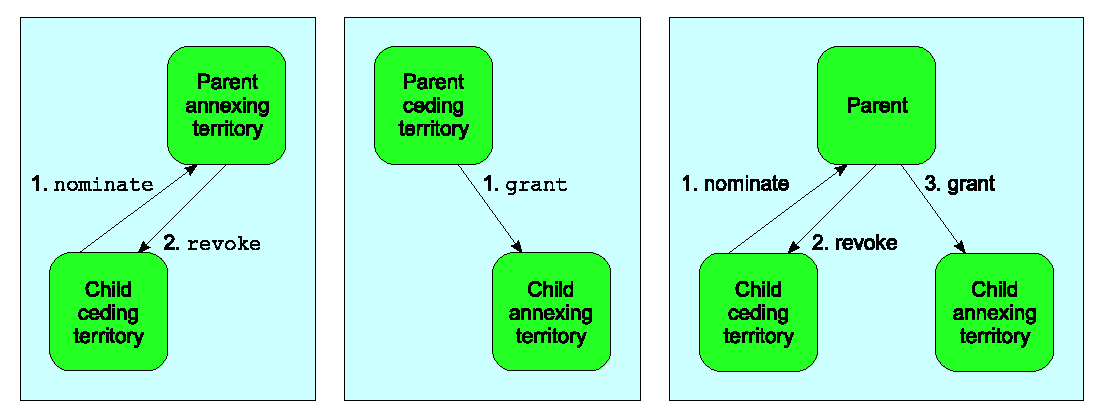
\includegraphics[width=100mm]{figures/grant-topdown}
\caption{Territory migrations are always driven by the parent in the namespace tree, which can annex a neighboring territory, cede territory to another envoy, or coordinates the transfer of a territory from one neighbor to another. For a child to initiate a transfer, it must send a \texttt{nominate} request to the parent, which then carries out the transfer.}
\label{fig:grant-topdown}
\end{figure}

\subsubsection{Transferring state}\label{sec:migrating-state}

When an envoy is granted a new territory, the first thing that it needs is a description of the boundaries. A territory is just a branch of the global namespace hierarchy, so it can be uniquly identified by its root pathname. In addition to that, the parent envoy sends a list of exits from the territory. An exit is a link to an already-established territory that branches off from the one being granted. Since the boundary description may include any number of exits, multiple messages may be required to transmit the full set.

The new owner also receives a full set of active file handles for the new territory. With the 9p protocol, a file handle may identify a opened or unopened files, file or directories used for \texttt{walk} or \texttt{stat} calls, or directories in the process of being read. To facilitate territory changes and transparent crash recovery, the envoy must be able to recreate any state needed to continue a directory read from the number of bytes returned so far in the sequence of reads. Transfers are relatively rare, and transfers that interrupt \texttt{readdir} sequences are even less common, so the prototype simply starts from the beginning and throws away enough data to find the appropriate place in the directory when the need arises.

Every element of state transferred to the new owner, including the boundaries and the file handles, has a counterpart maintained by a partner envoy that must be notified of the changes. The root name comes from the parent, which already knows about the transfer (since it initiated it), but the boundary exits and file handles require that notifications be sent to their respective envoys. The previous owner is a special case, and since it is also identified in the grant sequence, the new owner can safely assume that the old has completely adjusted to the new order of things and not explicitly notify it of each file handle and shared border the two have in common. Some may also be local to the new owner; good territory assignments regularly bring the territory to the main user, so this is a good result for file handles. For all others, the grant recipient sends a notification immediately, grouping multiple entries going to the same remote envoy when appropriate.

The other side of the process is having a territory ownership revoked. As with all such operations, the process is coordinated by the parent. Viewed strictly as a bilateral arrangement, every revoke appears to the child as a merger of a subtree into its parent, though for convenience it is given a hint about where the territory is going to end up.

A revoke operation works much like a grant operation in reverse: the envoy receives a revoke message identifying the root of the territory, and it responds by sending back the current borders and active file handles. It updates its own state for local file handles that become remote, but otherwise leaves updates to the new owner as described above. This is important for synchronizing the transfer with client requests, as detailed below.

Together with \texttt{nominate} messages, grant and revoke transactions give full flexibility for arranging territories. An envoy may cede part of its territory by granting it to a remote envoy and establishing a parent/child relationship with it. An owner may likewise cede its territory to the parent or to a third envoy by issuing a nominate request. Compound requests that carve up territories in more detail are not directly supported, though some could be simulated through sequences of transactions. In general, complicated control decisions made by a central player are avoided in preference to localized choices. The owner of a territory is the only envoy that knows the recent history of requests, and is thus best suited to make realignment decisions.

\subsubsection{Inflight operations}

Top-down coordination of synchronized transactions helps prevent deadlock, but other synchronization issues still exist in territory boundary changes. File operations may be at any stage of completion when the transfer begins, and all must complete successfully without interrupting the client.

The prototype is designed to favor simplicity over other virtues in complex transactions, and this is no exception. Each participant in a migration waits for all inflight transactions directly involving the territory in question to complete before locking it and queuing up any further incoming requests. When the transfer is complete, the lock is released and the queue examined. Significantly, a revoke transaction always completes after a grant (when the two are paired) and after all other envoys involved have been notified of the change. For some requests this will result in nothing more than a pause, while for others the immediate consequence is a failed result. The envoy may no longer recognize a file handle that has been transferred, and can do no more than send the request back to its originator to try again. Note that forwarding it as a special case is an option, but a dangerous one. The message could still end up at the wrong place due to bad timing (and a second transfer of the target), it would involve just as many network round trips (originator to old owner to new owner vs.\ originator to old owner followed by originator to new owner), and the new owner would reject the request anyway as coming from the wrong owner (recall that remote file handles are associated with the client's envoy).

\prettyref{fig:migrate-sync} illustrates a request that conflicts with a territory transfer. A request coming from a client's envoy that reaches its target before the territory is locked is allowed to run to completion. If it arrives after the lock, then it is suspended (this is true if the territory owner is the same as the client's envoy, or if it is remote). The revoke transaction only completes after the corresponding grant has completed and the client's envoy has been notified of the update, so when the old owner bounces the request back, the client's envoy knows the new forwarding address and can immediately retry the request with the new owner. If a request comes after a particular file handle has been updated but before the grant has completed, the new owner simply holds the request until the transfer transaction is complete, at which point it can safely start processing requests, even before the revoke operation has been finalized.

\begin{figure}[tp]
\centering
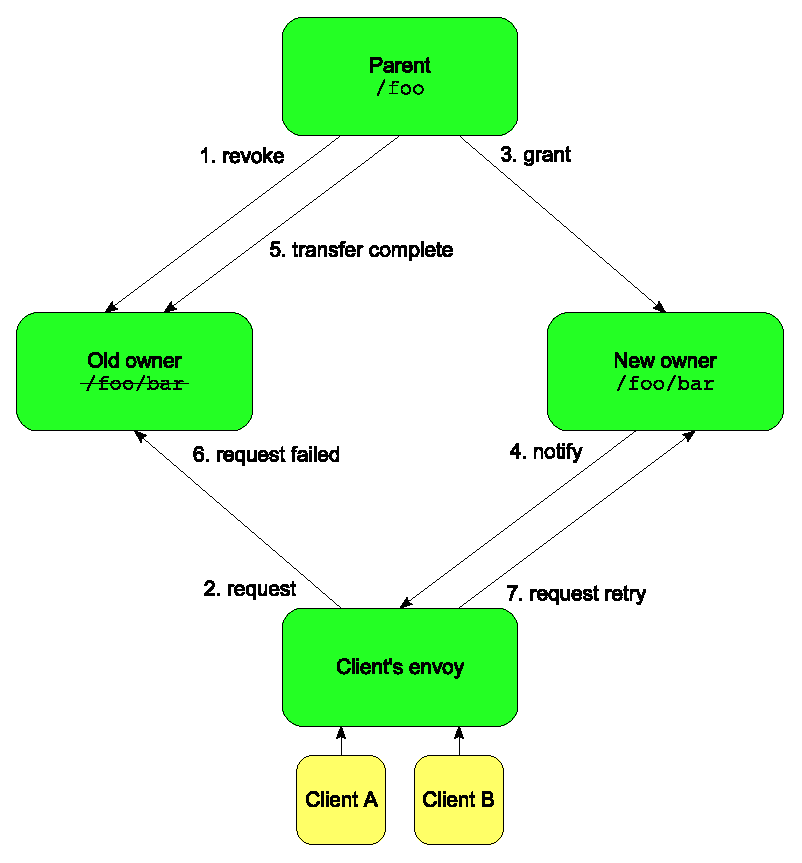
\includegraphics[width=100mm]{figures/migrate-sync}
\caption{The sequence of events when a client file request conflicts with a territory transfer.}
\label{fig:migrate-sync}
\end{figure}

\subsection{Limitations}

The prototype include some limitations that are artifacts of the implementation, rather than being inherent to the Envoy model. These are problems that can be solved with some routine engineering, and would need to be addressed in a production system. For the prototype, however, solving them would have added little value at the expense of extra complexity.

\subsubsection{Envoys as failure points}

The first issue is that a failing envoy loses all state for its local clients. This makes the failure of a single service affect all services on the same physical machine without an option for recovery. While services also depend on other node-wide management software, including the virtual machine manager, this is a dependency that could be removed.

The 9p protocol does not include any provision for recovering from a server failure, and the TCP connection used between the client and the envoy cannot be recovered transparently using standard network stacks. Both issues can be resolved by introducing a proxy between the client and the envoy (much as the envoy serves as a proxy for connections to remote envoys) that tracks the state of file handles, and is capable of restoring that state to a restarted envoy. Better yet, the client driver could be modified to maintain this state, and a recovery protocol introduced to synchronize and validate the state with a restarted envoy.

\subsubsection{Migrating clients}

A related problem is restoring state for VM instances that have been migrated to a different machine. With the current prototype, those instances will continue to send all requests to the envoy on the old machine, as they will not be aware of the migration. The envoys could easily transfer the state by employing a mechanism similar to that used to transfer territories, but a way to detect the migration would be necessary, probably through direct cooperation with the management process invoking the migration. The IP address of the new envoy would be different than the old, so some cooperation from the client would also be necessary to restart the TCP connection. Tricks involving the virtual network device connecting the client to the envoy may also be possible, but it is unlikely that the additional transparency gained would be worth the complexity introduced.

A related problem is virtual machines that are suspended to disk and restarted later, on either the same or a different physical machine. This can be viewed as another form of client migration, but from the client's perspective it more closely resembles the condition when the envoy fails and restarts. The solution proposed for that---clients retaining copies of file handle state and envoys validating and accepting it---would also be applicable here.

\subsubsection{Control of administrative directories}

For simplicity, territories control is only transferred starting at an image root, so all administrative directories are controlled by a single envoy. Traffic to these levels of the hierarchy are normally confined to mount requests and administrative actions, and for the latter most of the work for snapshot creation and removal is still done by territory owners.

Still, nothing precludes this area from being split up. Tracking authentication credentials and resolving the target of fork requests would become a bit more complex, but not substantially so.

The more serious issue is that the prototype cannot migrate control of the root to another envoy. The standard mechanism for migrating territories is applicable, but in addition all envoys would need to be notified of the change so that mount requests (which always start from the root of the namespace) could be properly routed. Straightforward solutions exist, but they were of little value in accomplishing the goals of the prototype and so were not pursued.

\section{Summary}
\chapter{Evaluation}\label{cha:evaluation}

synthetic workloads are a hard problem \cite{ganger95}

\section{Experimental setup}

\subsection{Test machines}

\subsection{Benchmarks}

\subsubsection{Linux source tree}
untar -- write test

tar > /dev/null -- read test

rsync -- 2nd read test

\subsubsection{Bonnie}

\section{Performance}

If the goal is to get stuff as local as possible, quantify the benefits of achieving that.

\subsection{Architectural costs}

userspace NFS

userspace 9p

envoy local dom0

envoy local domU

envoy remote dom0

envoy remote domU

cache: cold vs warm vs hot

\subsection{Fancy features}
\subsubsection{Forks}

cheap and fast---these always happen from a read-only snapshot

\subsubsection{Snapshots}

single territory, many territories

untar the kernel while a bunch of snapshots happen and measure the impact

\subsubsection{Territory migration}

\section{Scaling}
\subsection{Independence of private images}
\subsection{Degradation of a single host with many clients}
Shared image, and also private images on one machine

\section{Dynamic behaviour}

Test dynamic territory management, less about performance than behaviour

\subsection{Example scenarios}

shared image with (independent) home directories

2 log files in one directory

producer-consumer

\subsection{Sharing application}
distcc or something else that shares in a complex but predictable fashion

\subsection{Synthetic workloads}

probabilistic traffic driven to overlapping areas

\section{Case studies}

\subsection{Service deployment}
show sharing: boot one VM from cold cache, boot another based on same template

\subsection{Quantifying sharing}

SUSE10 upgrade, install services

compare image overlap

boot two related images (one cold and other warm) and compare with the same test for identical images

\section{Summary}
\chapter{Conclusion}\label{cha:conclusion}

\section{Future Work}
\subsection{Read-only leases}
\subsection{Custom protocol}
Cache at client for unshared objects, at envoy for shared
\subsection{Storage-informed load balancing}
\subsection{Object layer}
\subsection{Recovery}

\section{Summary}

% bibliography

\singlespace
\renewcommand{\bibname}{References}
\addcontentsline{toc}{chapter}{\bibname}
\bibliographystyle{plain}
\bibliography{references}

\end{document}
